% Options for packages loaded elsewhere
\PassOptionsToPackage{unicode}{hyperref}
\PassOptionsToPackage{hyphens}{url}
%
\documentclass[
]{article}
\usepackage{amsmath,amssymb}
\usepackage{lmodern}
\usepackage{iftex}
\ifPDFTeX
  \usepackage[T1]{fontenc}
  \usepackage[utf8]{inputenc}
  \usepackage{textcomp} % provide euro and other symbols
\else % if luatex or xetex
  \usepackage{unicode-math}
  \defaultfontfeatures{Scale=MatchLowercase}
  \defaultfontfeatures[\rmfamily]{Ligatures=TeX,Scale=1}
\fi
% Use upquote if available, for straight quotes in verbatim environments
\IfFileExists{upquote.sty}{\usepackage{upquote}}{}
\IfFileExists{microtype.sty}{% use microtype if available
  \usepackage[]{microtype}
  \UseMicrotypeSet[protrusion]{basicmath} % disable protrusion for tt fonts
}{}
\makeatletter
\@ifundefined{KOMAClassName}{% if non-KOMA class
  \IfFileExists{parskip.sty}{%
    \usepackage{parskip}
  }{% else
    \setlength{\parindent}{0pt}
    \setlength{\parskip}{6pt plus 2pt minus 1pt}}
}{% if KOMA class
  \KOMAoptions{parskip=half}}
\makeatother
\usepackage{xcolor}
\usepackage[margin=1in]{geometry}
\usepackage{color}
\usepackage{fancyvrb}
\newcommand{\VerbBar}{|}
\newcommand{\VERB}{\Verb[commandchars=\\\{\}]}
\DefineVerbatimEnvironment{Highlighting}{Verbatim}{commandchars=\\\{\}}
% Add ',fontsize=\small' for more characters per line
\usepackage{framed}
\definecolor{shadecolor}{RGB}{248,248,248}
\newenvironment{Shaded}{\begin{snugshade}}{\end{snugshade}}
\newcommand{\AlertTok}[1]{\textcolor[rgb]{0.94,0.16,0.16}{#1}}
\newcommand{\AnnotationTok}[1]{\textcolor[rgb]{0.56,0.35,0.01}{\textbf{\textit{#1}}}}
\newcommand{\AttributeTok}[1]{\textcolor[rgb]{0.77,0.63,0.00}{#1}}
\newcommand{\BaseNTok}[1]{\textcolor[rgb]{0.00,0.00,0.81}{#1}}
\newcommand{\BuiltInTok}[1]{#1}
\newcommand{\CharTok}[1]{\textcolor[rgb]{0.31,0.60,0.02}{#1}}
\newcommand{\CommentTok}[1]{\textcolor[rgb]{0.56,0.35,0.01}{\textit{#1}}}
\newcommand{\CommentVarTok}[1]{\textcolor[rgb]{0.56,0.35,0.01}{\textbf{\textit{#1}}}}
\newcommand{\ConstantTok}[1]{\textcolor[rgb]{0.00,0.00,0.00}{#1}}
\newcommand{\ControlFlowTok}[1]{\textcolor[rgb]{0.13,0.29,0.53}{\textbf{#1}}}
\newcommand{\DataTypeTok}[1]{\textcolor[rgb]{0.13,0.29,0.53}{#1}}
\newcommand{\DecValTok}[1]{\textcolor[rgb]{0.00,0.00,0.81}{#1}}
\newcommand{\DocumentationTok}[1]{\textcolor[rgb]{0.56,0.35,0.01}{\textbf{\textit{#1}}}}
\newcommand{\ErrorTok}[1]{\textcolor[rgb]{0.64,0.00,0.00}{\textbf{#1}}}
\newcommand{\ExtensionTok}[1]{#1}
\newcommand{\FloatTok}[1]{\textcolor[rgb]{0.00,0.00,0.81}{#1}}
\newcommand{\FunctionTok}[1]{\textcolor[rgb]{0.00,0.00,0.00}{#1}}
\newcommand{\ImportTok}[1]{#1}
\newcommand{\InformationTok}[1]{\textcolor[rgb]{0.56,0.35,0.01}{\textbf{\textit{#1}}}}
\newcommand{\KeywordTok}[1]{\textcolor[rgb]{0.13,0.29,0.53}{\textbf{#1}}}
\newcommand{\NormalTok}[1]{#1}
\newcommand{\OperatorTok}[1]{\textcolor[rgb]{0.81,0.36,0.00}{\textbf{#1}}}
\newcommand{\OtherTok}[1]{\textcolor[rgb]{0.56,0.35,0.01}{#1}}
\newcommand{\PreprocessorTok}[1]{\textcolor[rgb]{0.56,0.35,0.01}{\textit{#1}}}
\newcommand{\RegionMarkerTok}[1]{#1}
\newcommand{\SpecialCharTok}[1]{\textcolor[rgb]{0.00,0.00,0.00}{#1}}
\newcommand{\SpecialStringTok}[1]{\textcolor[rgb]{0.31,0.60,0.02}{#1}}
\newcommand{\StringTok}[1]{\textcolor[rgb]{0.31,0.60,0.02}{#1}}
\newcommand{\VariableTok}[1]{\textcolor[rgb]{0.00,0.00,0.00}{#1}}
\newcommand{\VerbatimStringTok}[1]{\textcolor[rgb]{0.31,0.60,0.02}{#1}}
\newcommand{\WarningTok}[1]{\textcolor[rgb]{0.56,0.35,0.01}{\textbf{\textit{#1}}}}
\usepackage{graphicx}
\makeatletter
\def\maxwidth{\ifdim\Gin@nat@width>\linewidth\linewidth\else\Gin@nat@width\fi}
\def\maxheight{\ifdim\Gin@nat@height>\textheight\textheight\else\Gin@nat@height\fi}
\makeatother
% Scale images if necessary, so that they will not overflow the page
% margins by default, and it is still possible to overwrite the defaults
% using explicit options in \includegraphics[width, height, ...]{}
\setkeys{Gin}{width=\maxwidth,height=\maxheight,keepaspectratio}
% Set default figure placement to htbp
\makeatletter
\def\fps@figure{htbp}
\makeatother
\setlength{\emergencystretch}{3em} % prevent overfull lines
\providecommand{\tightlist}{%
  \setlength{\itemsep}{0pt}\setlength{\parskip}{0pt}}
\setcounter{secnumdepth}{-\maxdimen} % remove section numbering
\ifLuaTeX
  \usepackage{selnolig}  % disable illegal ligatures
\fi
\IfFileExists{bookmark.sty}{\usepackage{bookmark}}{\usepackage{hyperref}}
\IfFileExists{xurl.sty}{\usepackage{xurl}}{} % add URL line breaks if available
\urlstyle{same} % disable monospaced font for URLs
\hypersetup{
  pdftitle={sustainability\_group3 - Trees},
  pdfauthor={Fabian Lüthard, Elisabeth Freimann, Simon Kohler},
  hidelinks,
  pdfcreator={LaTeX via pandoc}}

\title{sustainability\_group3 - Trees}
\author{Fabian Lüthard, Elisabeth Freimann, Simon Kohler}
\date{2023-02-06}

\begin{document}
\maketitle

{
\setcounter{tocdepth}{2}
\tableofcontents
}
\hypertarget{trees---trees---trees}{%
\section{TREES - TREES - TREES}\label{trees---trees---trees}}

\hypertarget{introduction}{%
\subsection{Introduction}\label{introduction}}

Vegetative cooling, or using plants to shield urban environments from
the sun's radiation, has been somewhat of a hot topic in recent years.
There has been plenty of research done in the field of vegetative
cooling for cities, such as, e.g.~a 2021 Europe-wide study by Schwaab et
al.~(\url{https://www.nature.com/articles/s41467-021-26768-w}), or a
simulation done on potential cooling effects of trees on Zurich's
Münsterhof by Kubilay et
al.~(\url{https://www.mdpi.com/2073-4433/11/12/1313} ). Both of these
studies find that urban trees do have at least a local cooling effect,
not only due to the shade that the trees provide, but also due to other
factors such as different evaporation or cool air flow as compared to
asphalt or concrete surfaces. While there has been ample more research
on the hyper-local effect to reduce or even eliminate heat islands, our
research focuses on the question of whether or not we can identify the
effect of the efforts of urban vegetative cooling in the city of Zurich
on a larger scale. Furthermore, we investigate if there is any
correlation with different factors in regards to air quality.

\hypertarget{goal-of-the-project}{%
\subsection{Goal of the project}\label{goal-of-the-project}}

We would like to prove that the planting of trees and the development of
green spaces in an urban environment have positive correlations with the
development of air quality indicators and a negative impact on
temperatures in the city of Zurich. This project will try to pinpoint
the effect trees have on these indicators. The results will be presented
in a way to inform politicians, urban developers as well as the public
about the impact that a more green city could have on our everyday
lives. While there are a number of potential factors, both local and
national/global, can have a significant impact on the climate and for
this research we are choosing to focus on data from Zürich in regards to
air quality, temperature information and the tree inventory. Further
factors are described using sources, but are not included in the data
analysis. To clarify our project goal and narrow it down we drew the
following picture:

\begin{figure}
\centering
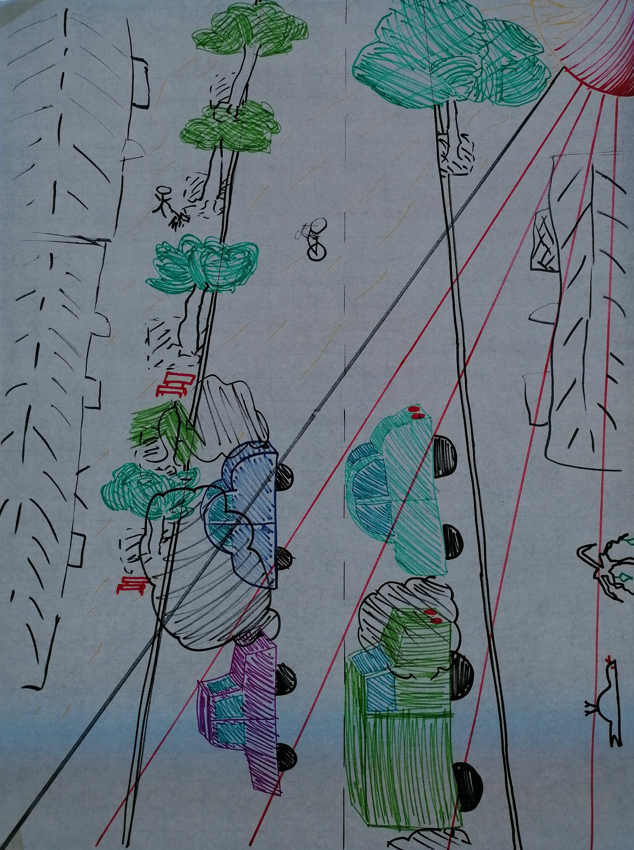
\includegraphics{../images/trees_vs_Pollution.png}
\caption{Target Picture}
\end{figure}

It shows two potential futures for Zürich. One with more green spaces
and one with more urban wasteland. The idea of the project is to find
out how much the trees and green spaces actually impact the city of
Zürich in regard to temperature and air pollution.

Scope \& Limitations Our data sets are limited to the trees planted by
garden and forestation services of the municipality of Zurich (Grün
Stadt Zürich), and only include roadside and park trees. The effect of
local de- or reforestation thus cannot be accounted for. Furthermore,
temperature data was taken from roadside stations that could themselves
potentially be located within heat islands. It also needs to be noted,
that we did not take existing trees into account, but only looked at
whether or not we could see a (lagged) correlation between newly planted
trees and temperature development within the districts that our
measurement stations were located in. Furthermore, as our analysis moves
beyond a micro-scale, there are many more factors that we cannot control
for, both on the local and macro-environmental level. A factor that we
did not control for, which could have large implications on the macro
scale of temperature, is the potential disappearance of undeveloped land
and urban expansion. Additionally, an analysis of building materials
used was also out of the scope of this analysis. The temporal scope of
our data is limited to the span between 1983 and 2022. To visualize the
scope of our project, we have created a systems view that can be seen
below.

\begin{figure}
\centering
\includegraphics{../images/loopy.gif}
\caption{Systems View}
\end{figure}

\hypertarget{stakeholders}{%
\subsubsection{Stakeholders}\label{stakeholders}}

To ensure we include all potential stakeholders in our project at the
appropriate level we created the following stakeholder map:

\begin{figure}
\centering
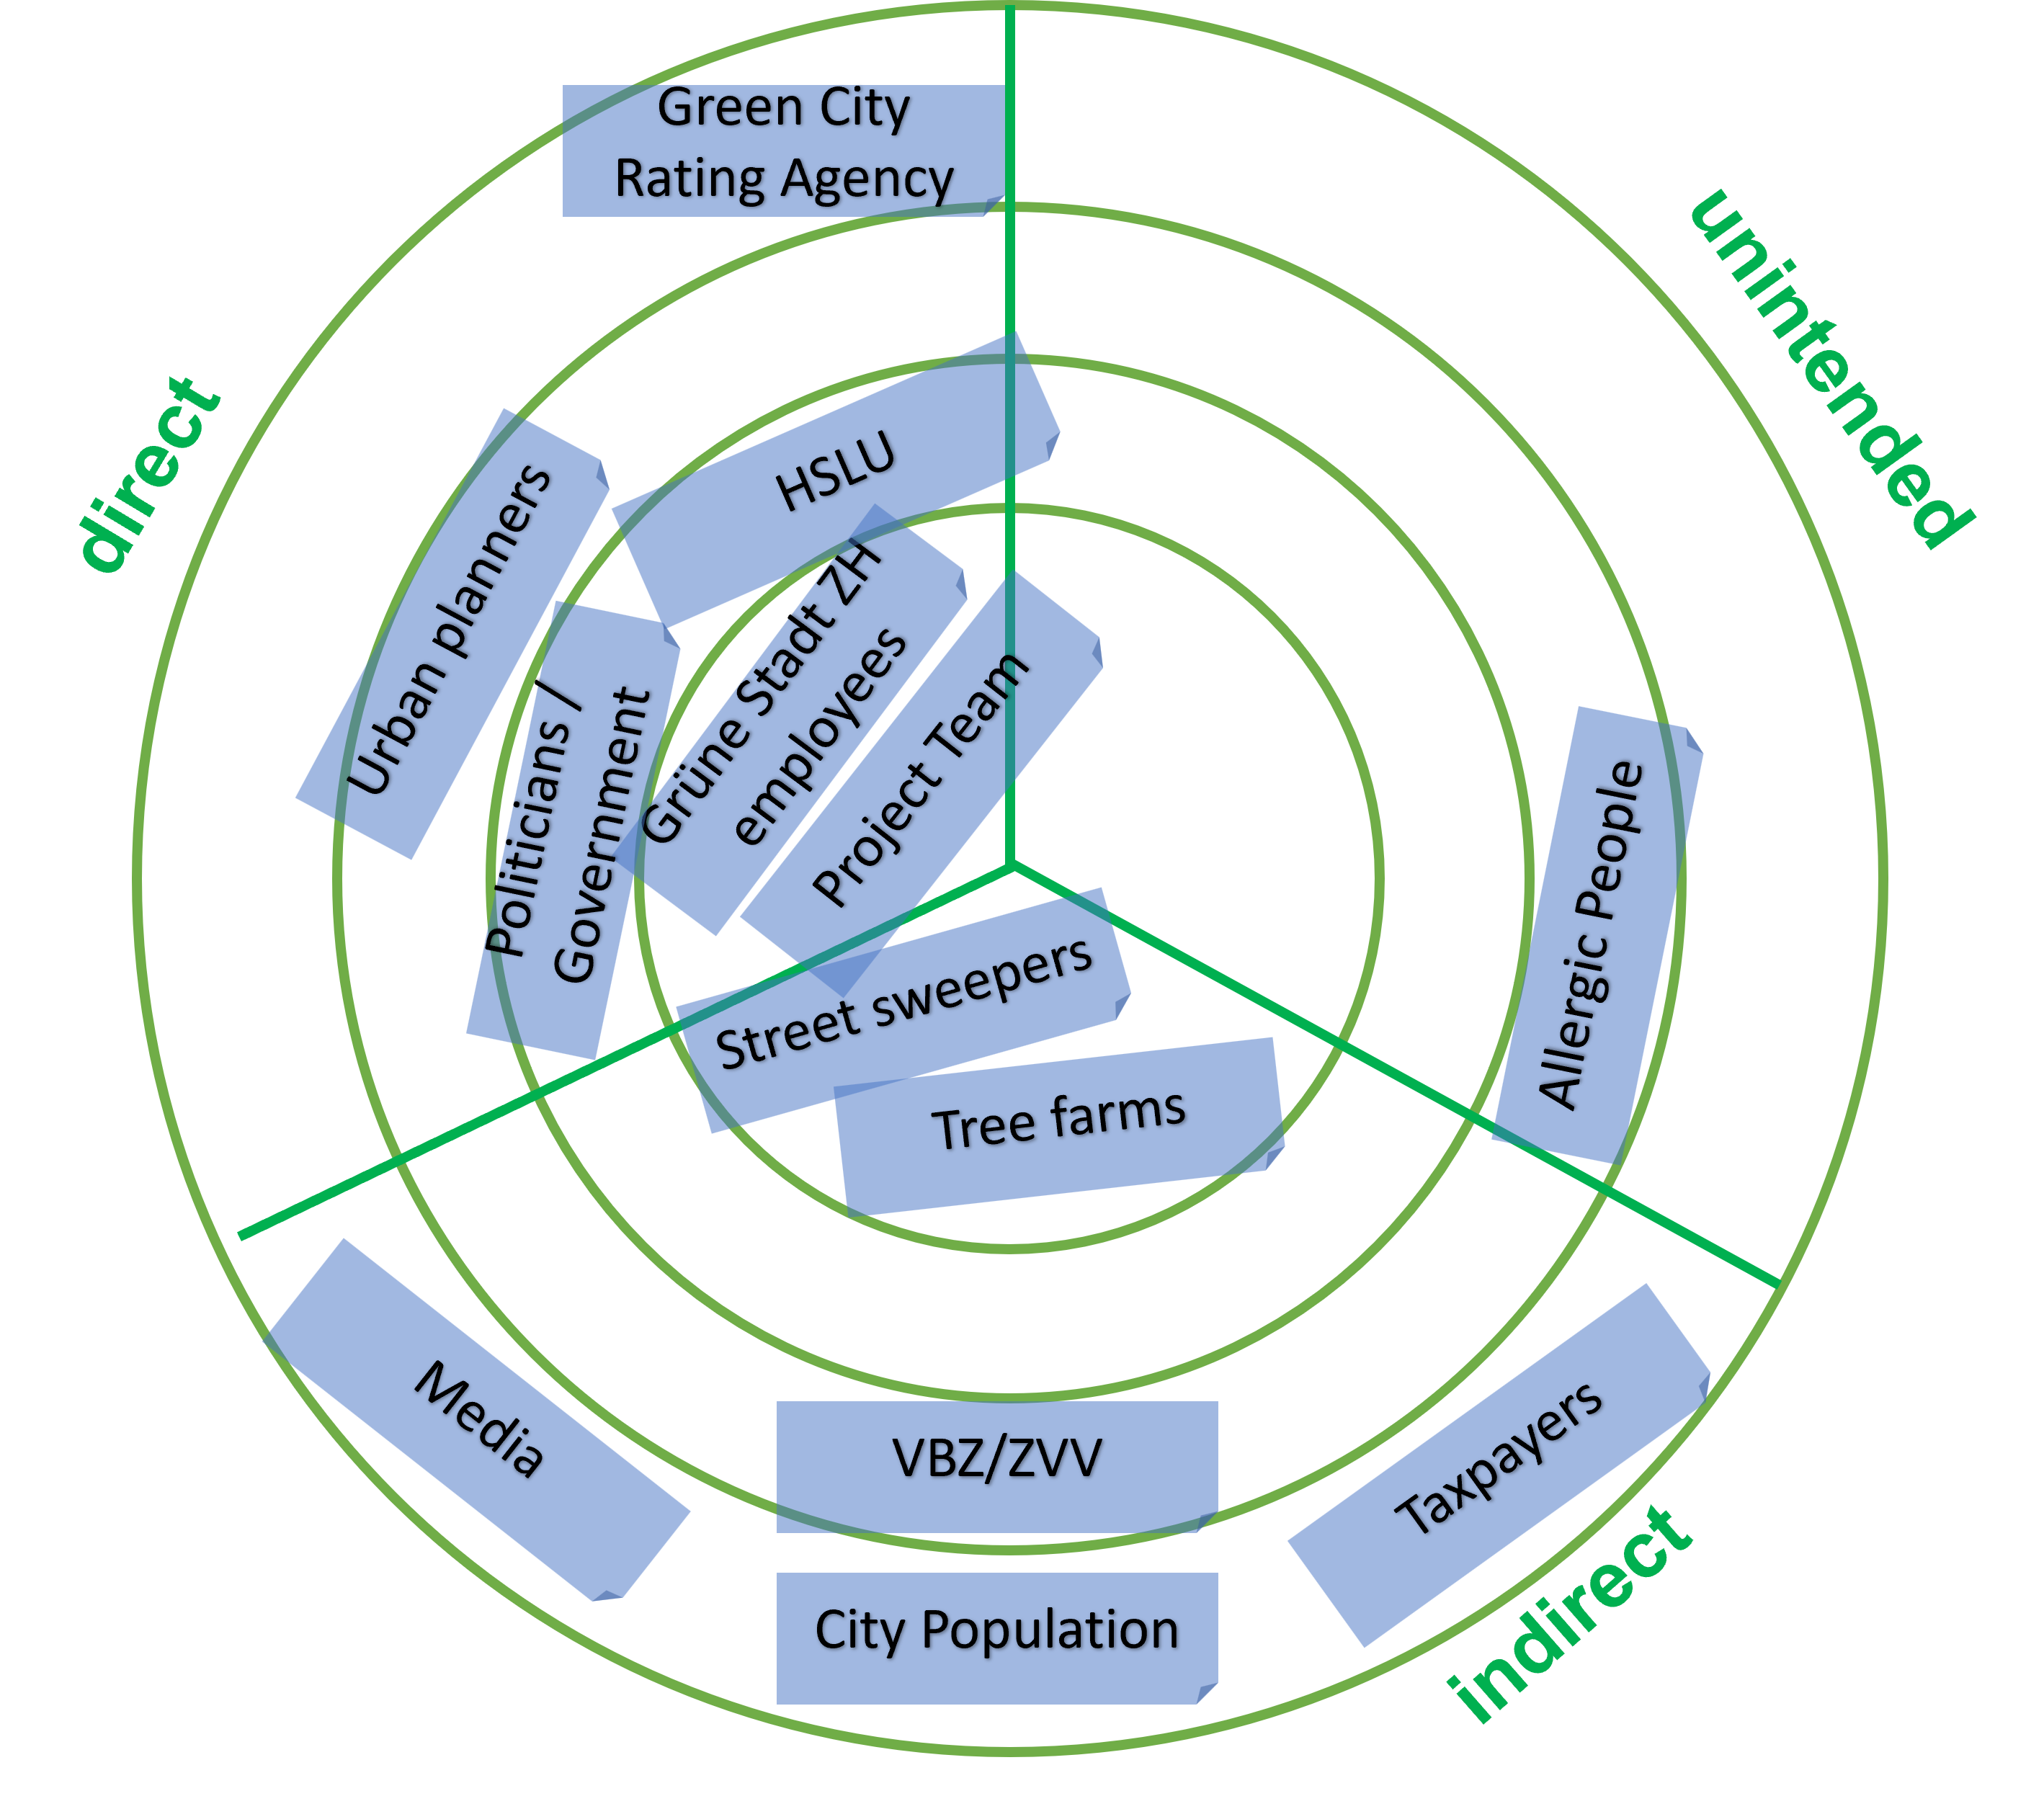
\includegraphics{../images/Stakeholders.png}
\caption{Stakeholders}
\end{figure}

We sorted them into three possible categories: ``direct'', ``indirect'',
``unintended''. Our main target is to work together with Grüne Stadt
Zürich and convince the politicians, the government and urban planners
on the benefits of a greener city. Indirectly involved would be street
sweepers, who have to deal with more leafs etc on the streets, and tree
farms, who would be relied upon to provide the trees. The stakeholder
map list further stakeholders who need to be considered if the proposed
changes would be implemented. It is also very possible and even likely
that additional stakeholders will have to be considered during the
project.

\hypertarget{big-picture-embedding-in-the-sustainable-development-goals-sdg}{%
\subsection{Big Picture: Embedding in the Sustainable Development Goals
(SDG)}\label{big-picture-embedding-in-the-sustainable-development-goals-sdg}}

The SDGs lay out the goals that the global community (United Nations
General Assembly in 2015) has agreed on. Total there are 17 goals and
they range from 1. No poverty to 17. Partnerships for the goals and
include social, economic and environmental targets. For the research we
have identified the relevant goals and put them into the three different
categories: Risk, Opportunity and Intended.

\includegraphics{../images/sdg.png} As can be seen, the intended target
for our research is to help achieve the goal number 3. Good health and
well being. This can be achieved if we can prove a correlation between
the amount of trees in a region and an improvement in air quality, which
could then lead to increase of planting of new trees in Zürich as well
as a reduction of concrete wastelands in favor of green spaces. There
are a number opportunities as well in regards to climate action,
economic growth and affordable and clean energy. The are only limited
risks that this project has. However it is imaginable that the
improvement in air quality in certain areas could lead to a increase in
inequalities between the rich and poor. It is also important to always
be responsible and think of possible unintended consequences while
planning for new green zones and planting new trees.

\hypertarget{data-sources}{%
\subsection{Data sources}\label{data-sources}}

For the research there are three different data sets needed: Air quality
information, temperature data, and a tree cadastre. All of these three
data sets are publicly available. Following is a quick overview over the
different data sets:

\hypertarget{air-quality}{%
\subsubsection{Air quality}\label{air-quality}}

Format: csv\\
Number of rows: 283'763\\
Number of variables: 8 (most important: date, location, type of
measurement, value)\\
Source:
\url{https://data.stadt-zuerich.ch/dataset/ugz_luftschadstoffmessung_stundenwerte}

\hypertarget{meteo-1-zurich-city}{%
\subsubsection{Meteo 1 (Zurich City)}\label{meteo-1-zurich-city}}

Format: csv\\
Number of rows: 4'747\\
Number of variables: 17 (most important: date, temperature, location)\\
Source:
\url{https://opendata.swiss/de/dataset/taglich-aktualisierte-meteodaten-seit-1992}

\hypertarget{meteo-2-fluntern-reference-station}{%
\subsubsection{Meteo 2 (Fluntern Reference
Station)}\label{meteo-2-fluntern-reference-station}}

Format: csv\\
Number of rows: 15706 Number of variables: 20 (most important: date,
temperature, location)\\
Source: \url{https://gate.meteoswiss.ch/idaweb}

\hypertarget{tree-cadastre}{%
\subsubsection{Tree Cadastre}\label{tree-cadastre}}

Format: csv\\
Number of rows: 36'239\\
Number of variables: 17 (most important: year of planting, diameter of
crown, district)\\
Source: \url{https://data.stadt-zuerich.ch/dataset/geo_baumkataster}

\hypertarget{data-preparation}{%
\subsection{Data preparation}\label{data-preparation}}

In this step we collected the three data sets and prepared them so that
they are for use in the analysis. To achieve this, certain changes to
the data were necessary to facilitate an informative analysis.

First we loaded the tree cadastre data and wrangled the data to get
additional information such as the amount of trees per year and the
number of trees by district.

\begin{Shaded}
\begin{Highlighting}[]
\NormalTok{d.trees }\OtherTok{\textless{}{-}} \FunctionTok{read.csv}\NormalTok{(}\StringTok{\textquotesingle{}../datasets/gsz.baumkataster\_baumstandorte.csv\textquotesingle{}}\NormalTok{, }\AttributeTok{encoding =} \StringTok{"UTF{-}8"}\NormalTok{)}
\FunctionTok{names}\NormalTok{(d.trees)[}\DecValTok{1}\NormalTok{] }\OtherTok{\textless{}{-}} \StringTok{"objid"} 
\CommentTok{\#head(trees)}
\CommentTok{\#str(trees)}


\CommentTok{\#Wrangling and mutating tree data}

\CommentTok{\# trees by year}
\NormalTok{tree\_ts }\OtherTok{\textless{}{-}}\NormalTok{ d.trees }\SpecialCharTok{\%\textgreater{}\%}
\NormalTok{  dplyr}\SpecialCharTok{::}\FunctionTok{select}\NormalTok{(pflanzjahr) }\SpecialCharTok{\%\textgreater{}\%}
  \FunctionTok{filter}\NormalTok{(pflanzjahr }\SpecialCharTok{\textgreater{}} \DecValTok{1980}\NormalTok{) }\SpecialCharTok{\%\textgreater{}\%}
  \FunctionTok{group\_by}\NormalTok{(pflanzjahr) }\SpecialCharTok{\%\textgreater{}\%}
  \FunctionTok{summarise}\NormalTok{(}\AttributeTok{count =} \FunctionTok{n}\NormalTok{())}

\CommentTok{\# Trees by district}
\NormalTok{tree\_quartier }\OtherTok{\textless{}{-}}\NormalTok{ d.trees }\SpecialCharTok{\%\textgreater{}\%}
\NormalTok{  dplyr}\SpecialCharTok{::}\FunctionTok{select}\NormalTok{(pflanzjahr, objid, quartier) }\SpecialCharTok{\%\textgreater{}\%}
  \FunctionTok{filter}\NormalTok{(pflanzjahr }\SpecialCharTok{\textgreater{}} \DecValTok{1980}\NormalTok{) }\SpecialCharTok{\%\textgreater{}\%}
  \FunctionTok{group\_by}\NormalTok{(pflanzjahr, quartier) }\SpecialCharTok{\%\textgreater{}\%}
  \FunctionTok{summarise}\NormalTok{(}\AttributeTok{count =} \FunctionTok{n}\NormalTok{())}


\CommentTok{\# sum of trees}
\NormalTok{tree\_ts\_sum }\OtherTok{\textless{}{-}}\NormalTok{ tree\_ts }\SpecialCharTok{\%\textgreater{}\%}
 \FunctionTok{mutate}\NormalTok{(}\AttributeTok{sum\_trees =} \FunctionTok{cumsum}\NormalTok{(count))}


\CommentTok{\# Trees by district, year}
\NormalTok{tree\_quartier\_year\_full }\OtherTok{\textless{}{-}}\NormalTok{ d.trees }\SpecialCharTok{\%\textgreater{}\%}
\NormalTok{  dplyr}\SpecialCharTok{::}\FunctionTok{select}\NormalTok{(pflanzjahr, quartier, kronendurchmesser) }\SpecialCharTok{\%\textgreater{}\%}
  \FunctionTok{filter}\NormalTok{(pflanzjahr }\SpecialCharTok{\textgreater{}} \DecValTok{1980}\NormalTok{) }\SpecialCharTok{\%\textgreater{}\%}
  \FunctionTok{group\_by}\NormalTok{(pflanzjahr, quartier) }\SpecialCharTok{\%\textgreater{}\%}
  \FunctionTok{summarise}\NormalTok{(}\AttributeTok{count =} \FunctionTok{n}\NormalTok{(), }\AttributeTok{sum\_crown =} \FunctionTok{sum}\NormalTok{(kronendurchmesser))}

\CommentTok{\# trees by year}
\NormalTok{tree\_year }\OtherTok{\textless{}{-}}\NormalTok{ d.trees }\SpecialCharTok{\%\textgreater{}\%}
\NormalTok{  dplyr}\SpecialCharTok{::}\FunctionTok{select}\NormalTok{(pflanzjahr, kronendurchmesser) }\SpecialCharTok{\%\textgreater{}\%}
  \FunctionTok{filter}\NormalTok{(pflanzjahr }\SpecialCharTok{\textgreater{}} \DecValTok{1980}\NormalTok{) }\SpecialCharTok{\%\textgreater{}\%}
  \FunctionTok{group\_by}\NormalTok{(pflanzjahr) }\SpecialCharTok{\%\textgreater{}\%}
  \FunctionTok{summarise}\NormalTok{(}\AttributeTok{tree\_count =} \FunctionTok{n}\NormalTok{(), }\AttributeTok{crown\_sum =} \FunctionTok{sum}\NormalTok{(kronendurchmesser))}

\NormalTok{tree\_year\_sum }\OtherTok{\textless{}{-}}\NormalTok{ tree\_year }\SpecialCharTok{\%\textgreater{}\%}
  \FunctionTok{mutate}\NormalTok{(}\AttributeTok{cum\_trees =} \FunctionTok{cumsum}\NormalTok{(tree\_count)) }\SpecialCharTok{\%\textgreater{}\%}
  \FunctionTok{mutate}\NormalTok{(}\AttributeTok{cum\_crown =} \FunctionTok{cumsum}\NormalTok{(crown\_sum))}
\end{Highlighting}
\end{Shaded}

Next we load all the temperature information from the meteo data set.
While this data set includes other information such as rain duration we
will only use the temperature, as it seems unlikely that the amount of
trees significantly impact the rain fall in an area.

\begin{Shaded}
\begin{Highlighting}[]
\NormalTok{filenames.meteo }\OtherTok{\textless{}{-}} \FunctionTok{list.files}\NormalTok{(}\AttributeTok{path =} \StringTok{"../datasets/meteo/"}\NormalTok{, }\AttributeTok{pattern =} \StringTok{"*.csv"}\NormalTok{, }\AttributeTok{full.names =} \ConstantTok{TRUE}\NormalTok{)}
\NormalTok{data\_list.meteo }\OtherTok{\textless{}{-}} \FunctionTok{lapply}\NormalTok{(filenames.meteo, read.csv)}
\CommentTok{\# Combine the data frames in the list into a single data frame}
\NormalTok{meteo }\OtherTok{\textless{}{-}} \FunctionTok{do.call}\NormalTok{(rbind, data\_list.meteo)}

\FunctionTok{names}\NormalTok{(meteo)[}\DecValTok{1}\NormalTok{] }\OtherTok{\textless{}{-}} \StringTok{"Date"}
\NormalTok{meteo}\SpecialCharTok{$}\NormalTok{Date }\OtherTok{\textless{}{-}} \FunctionTok{format}\NormalTok{(}\FunctionTok{as.Date}\NormalTok{(meteo}\SpecialCharTok{$}\NormalTok{Date), }\AttributeTok{format =} \StringTok{"\%Y{-}\%m{-}\%d"}\NormalTok{)}

\CommentTok{\# Datensatz mit Temperatur und Globalstrahlung pro Messstation}
\NormalTok{meteo.extr }\OtherTok{\textless{}{-}}\NormalTok{ meteo }\SpecialCharTok{\%\textgreater{}\%}
  \FunctionTok{filter}\NormalTok{(Parameter }\SpecialCharTok{==} \StringTok{"T"} \SpecialCharTok{|}\NormalTok{ Parameter }\SpecialCharTok{==} \StringTok{"StrGlo"} \SpecialCharTok{|}\NormalTok{ Parameter }\SpecialCharTok{==}\StringTok{"T\_max\_h1"}\NormalTok{)}
\NormalTok{meteo.extr}\SpecialCharTok{$}\NormalTok{Jahr }\OtherTok{\textless{}{-}} \FunctionTok{year}\NormalTok{(meteo.extr}\SpecialCharTok{$}\NormalTok{Date)}

\CommentTok{\# weiter mit "normalem" Meteodatensatz}
\NormalTok{meteo }\OtherTok{\textless{}{-}}\NormalTok{ meteo[meteo}\SpecialCharTok{$}\NormalTok{Standort}\SpecialCharTok{==}\StringTok{"Zch\_Stampfenbachstrasse"}\NormalTok{,]}
\NormalTok{meteo }\OtherTok{\textless{}{-}}\NormalTok{ meteo }\SpecialCharTok{\%\textgreater{}\%} 
  \FunctionTok{select}\NormalTok{(}\FunctionTok{c}\NormalTok{(}\StringTok{"Date"}\NormalTok{,}\StringTok{"Parameter"}\NormalTok{,}\StringTok{"Wert"}\NormalTok{)) }\SpecialCharTok{\%\textgreater{}\%}
  \FunctionTok{pivot\_wider}\NormalTok{(}\AttributeTok{id\_cols =} \StringTok{"Date"}\NormalTok{,}\AttributeTok{names\_from =} \StringTok{"Parameter"}\NormalTok{,}\AttributeTok{values\_from =} \StringTok{"Wert"}\NormalTok{) }\SpecialCharTok{\%\textgreater{}\%}
  \FunctionTok{select}\NormalTok{(}\FunctionTok{c}\NormalTok{(}\StringTok{"Date"}\NormalTok{,}\StringTok{"T"}\NormalTok{,}\StringTok{"RainDur"}\NormalTok{,}\StringTok{"p"}\NormalTok{))}

\NormalTok{meteo}\SpecialCharTok{$}\NormalTok{Date }\OtherTok{\textless{}{-}} \FunctionTok{ymd}\NormalTok{(meteo}\SpecialCharTok{$}\NormalTok{Date)}

\FunctionTok{head}\NormalTok{(meteo)}
\end{Highlighting}
\end{Shaded}

\begin{verbatim}
## # A tibble: 6 x 4
##   Date           T RainDur     p
##   <date>     <dbl>   <dbl> <dbl>
## 1 1992-07-01  19.0      NA  963.
## 2 1992-07-02  18.4      NA  965.
## 3 1992-07-03  21.5      NA  965.
## 4 1992-07-04  17.5      NA  961.
## 5 1992-07-05  15.6      NA  958.
## 6 1992-07-06  17        NA  960.
\end{verbatim}

Lastly the air quality data is loaded. While there are multiple location
were air quality was measured not every station measured each variable.
They also were not all built at the same time.

\begin{Shaded}
\begin{Highlighting}[]
\NormalTok{filenames.air }\OtherTok{\textless{}{-}} \FunctionTok{list.files}\NormalTok{(}\AttributeTok{path =} \StringTok{"../datasets/air/"}\NormalTok{, }\AttributeTok{pattern =} \StringTok{"*.csv"}\NormalTok{, }\AttributeTok{full.names =} \ConstantTok{TRUE}\NormalTok{)}
\NormalTok{data\_list.air }\OtherTok{\textless{}{-}} \FunctionTok{lapply}\NormalTok{(filenames.air, read.csv)}
\CommentTok{\# Combine the data frames in the list into a single data frame}
\NormalTok{air }\OtherTok{\textless{}{-}} \FunctionTok{do.call}\NormalTok{(rbind, data\_list.air)}
\FunctionTok{names}\NormalTok{(air)[}\DecValTok{1}\NormalTok{] }\OtherTok{\textless{}{-}} \StringTok{"Date"}
\NormalTok{air}\SpecialCharTok{$}\NormalTok{Date }\OtherTok{\textless{}{-}} \FunctionTok{as.Date}\NormalTok{(}\FunctionTok{format}\NormalTok{(air}\SpecialCharTok{$}\NormalTok{Date), }\StringTok{"\%Y{-}\%m{-}\%d"}\NormalTok{)}
\CommentTok{\# add column Jahr}
\NormalTok{air}\SpecialCharTok{$}\NormalTok{Jahr }\OtherTok{\textless{}{-}} \FunctionTok{as.numeric}\NormalTok{(}\FunctionTok{format}\NormalTok{(air}\SpecialCharTok{$}\NormalTok{Date,}\StringTok{\textquotesingle{}\%Y\textquotesingle{}}\NormalTok{))}
\FunctionTok{head}\NormalTok{(air)}
\end{Highlighting}
\end{Shaded}

\begin{verbatim}
##         Date                Standort Parameter Intervall Einheit   Wert
## 1 1983-01-01 Zch_Stampfenbachstrasse        CO        d1   mg/m3   4.10
## 2 1983-01-01 Zch_Stampfenbachstrasse       NO2        d1   µg/m3  68.80
## 3 1983-01-01 Zch_Stampfenbachstrasse        NO        d1   µg/m3 214.73
## 4 1983-01-01 Zch_Stampfenbachstrasse       NOx        d1     ppb 208.14
## 5 1983-01-01 Zch_Stampfenbachstrasse       SO2        d1   µg/m3 133.26
## 6 1983-01-02 Zch_Stampfenbachstrasse        CO        d1   mg/m3   3.77
##      Status Jahr
## 1 bereinigt 1983
## 2 bereinigt 1983
## 3 bereinigt 1983
## 4 bereinigt 1983
## 5 bereinigt 1983
## 6 bereinigt 1983
\end{verbatim}

\begin{Shaded}
\begin{Highlighting}[]
\NormalTok{air.wide }\OtherTok{\textless{}{-}}\NormalTok{ air }\SpecialCharTok{\%\textgreater{}\%} 
  \FunctionTok{filter}\NormalTok{(Standort }\SpecialCharTok{==} \StringTok{"Zch\_Stampfenbachstrasse"}\NormalTok{) }\SpecialCharTok{\%\textgreater{}\%}
  \FunctionTok{select}\NormalTok{(}\FunctionTok{c}\NormalTok{(}\StringTok{"Date"}\NormalTok{, }\StringTok{"Parameter"}\NormalTok{, }\StringTok{"Wert"}\NormalTok{)) }\SpecialCharTok{\%\textgreater{}\%}
  \FunctionTok{pivot\_wider}\NormalTok{(}\AttributeTok{id\_cols =} \StringTok{"Date"}\NormalTok{, }\AttributeTok{names\_from =} \StringTok{"Parameter"}\NormalTok{, }\AttributeTok{values\_from =} \StringTok{"Wert"}\NormalTok{)}

\NormalTok{air.short }\OtherTok{\textless{}{-}}\NormalTok{ air[air}\SpecialCharTok{$}\NormalTok{Standort}\SpecialCharTok{==}\StringTok{"Zch\_Stampfenbachstrasse"}\NormalTok{,]}

\NormalTok{air.short }\OtherTok{\textless{}{-}}\NormalTok{ air.short }\SpecialCharTok{\%\textgreater{}\%}
  \FunctionTok{select}\NormalTok{(}\FunctionTok{c}\NormalTok{(}\StringTok{"Date"}\NormalTok{, }\StringTok{"Parameter"}\NormalTok{, }\StringTok{"Wert"}\NormalTok{)) }\SpecialCharTok{\%\textgreater{}\%}
  \FunctionTok{pivot\_wider}\NormalTok{(}\AttributeTok{id\_cols =} \StringTok{"Date"}\NormalTok{,}\AttributeTok{names\_from =} \StringTok{"Parameter"}\NormalTok{,}\AttributeTok{values\_from =} \StringTok{"Wert"}\NormalTok{)}

\NormalTok{keep }\OtherTok{\textless{}{-}} \FunctionTok{c}\NormalTok{(}\StringTok{"Date"}\NormalTok{, }\StringTok{"CO"}\NormalTok{, }\StringTok{"NOx"}\NormalTok{)}
\NormalTok{air.short }\OtherTok{\textless{}{-}}\NormalTok{ air.short[keep]}
\NormalTok{keep }\OtherTok{\textless{}{-}} \FunctionTok{c}\NormalTok{(}\StringTok{"Date"}\NormalTok{, }\StringTok{"CO"}\NormalTok{)}
\NormalTok{air.co }\OtherTok{\textless{}{-}}\NormalTok{ air.short[keep]}
\NormalTok{keep }\OtherTok{\textless{}{-}} \FunctionTok{c}\NormalTok{(}\StringTok{"Date"}\NormalTok{, }\StringTok{"NOx"}\NormalTok{)}
\NormalTok{air.NOx }\OtherTok{\textless{}{-}}\NormalTok{ air.short[keep]}
\CommentTok{\#air.NOx \textless{}{-} air["NOx"] \textless{}{-} log(air["NOx"])}
\end{Highlighting}
\end{Shaded}

\hfill\break

\hypertarget{insights-into-our-datasets}{%
\section{Insights into our datasets}\label{insights-into-our-datasets}}

\hfill\break

To gain insights from the available information we have created a number
of graphical overviews. These already show preliminary results of our
analysis.

\hfill\break

\hypertarget{air-quality-in-zuxfcrich-and-its-development-over-the-years}{%
\subsection{Air quality in Zürich and its development over the
years}\label{air-quality-in-zuxfcrich-and-its-development-over-the-years}}

\hfill\break

\hypertarget{daily-development-of-carbon-monoxide-and-nitrogen-oxides}{%
\subsubsection{Daily development of Carbon Monoxide and Nitrogen
Oxides}\label{daily-development-of-carbon-monoxide-and-nitrogen-oxides}}

\begin{figure}

{\centering 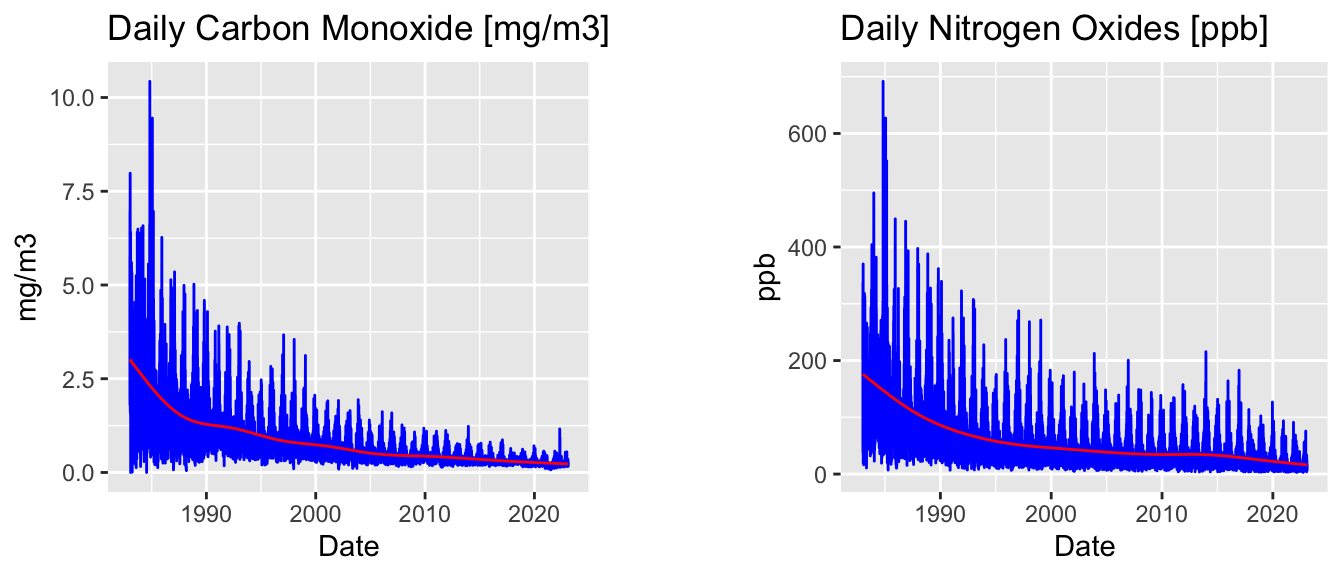
\includegraphics[width=0.9\linewidth]{sustainability_group_files/figure-latex/plot_air-1} 

}

\caption{Fig. nnn: Daily CO and NOx}\label{fig:plot_air}
\end{figure}

A first visual inspection of carbon monoxide and nitrogen oxides as
illustrated in figure nnn shows a reduction of both, CO and NOx, as of
1983 up to 2022. The trend line in red shows a significant improvement
especially in the Eighties and early Nineties. It is unlikely that trees
are the only factor influencing this improvement. Rather other factors
such as new laws and regulations play a major role. In addition, in this
timeframe, the cars were equipped with catalysts which mainly reduce
carbon monoxide, hydrocarbon and nitrogen oxyds. Searching the internet
for explanations to which we could refer didn't lead to any results, as
most time series only start as of 1990. Additional potential influencing
factors are mentioned in nnn.

\hfill\break
\hfill\break
--\textgreater{} hier die Referenz auf Loopy Kapitel\\
\strut \\

The same data depicted as boxplots and summarized per year confirms the
improvement of air quaility as well as the trend and the maximum values.

\begin{figure}

{\centering 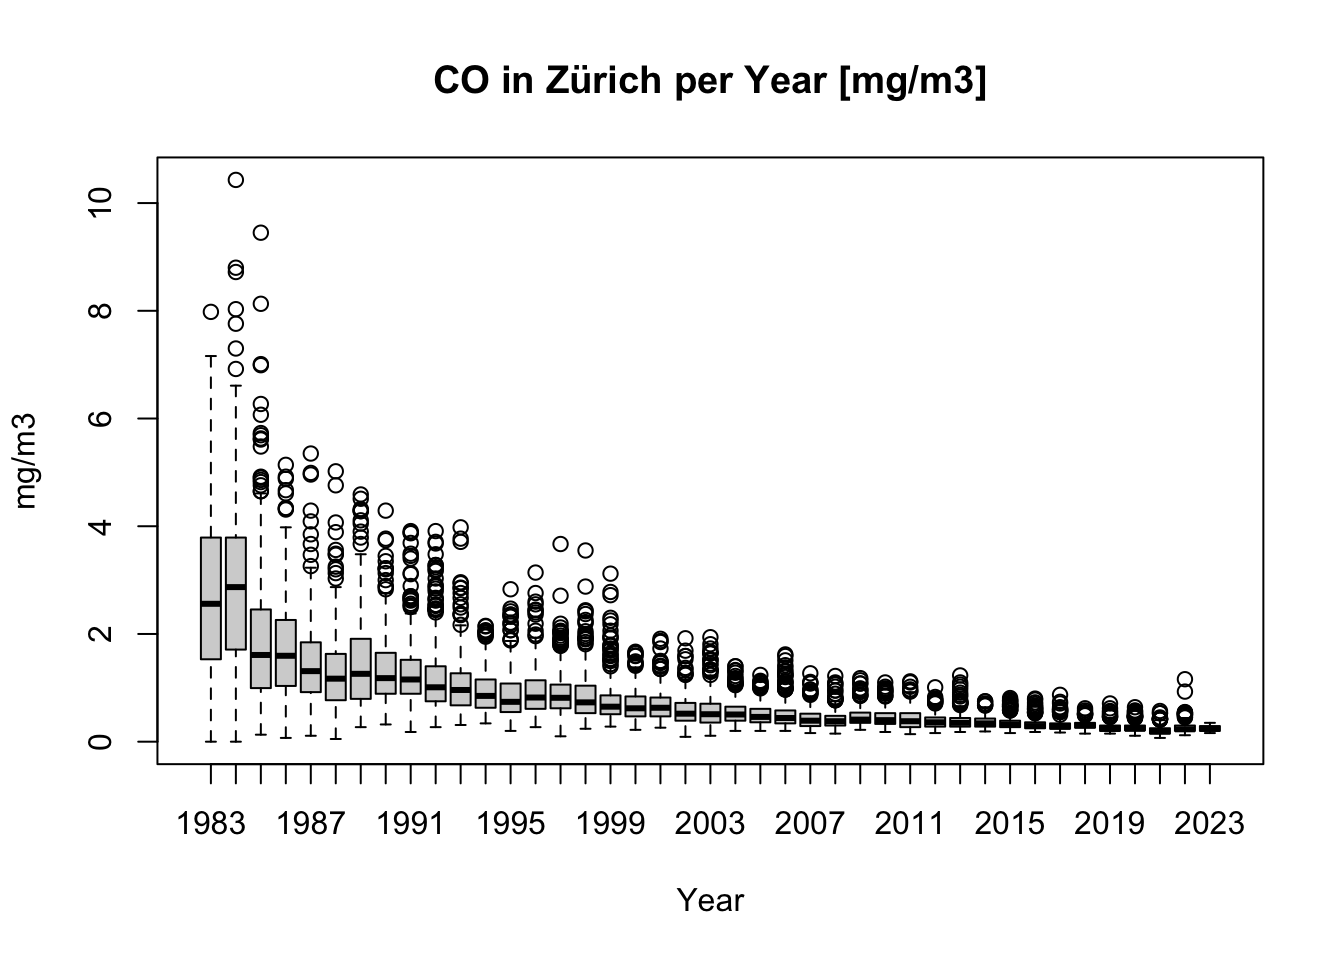
\includegraphics[width=0.45\linewidth]{sustainability_group_files/figure-latex/air.boxplots-1} 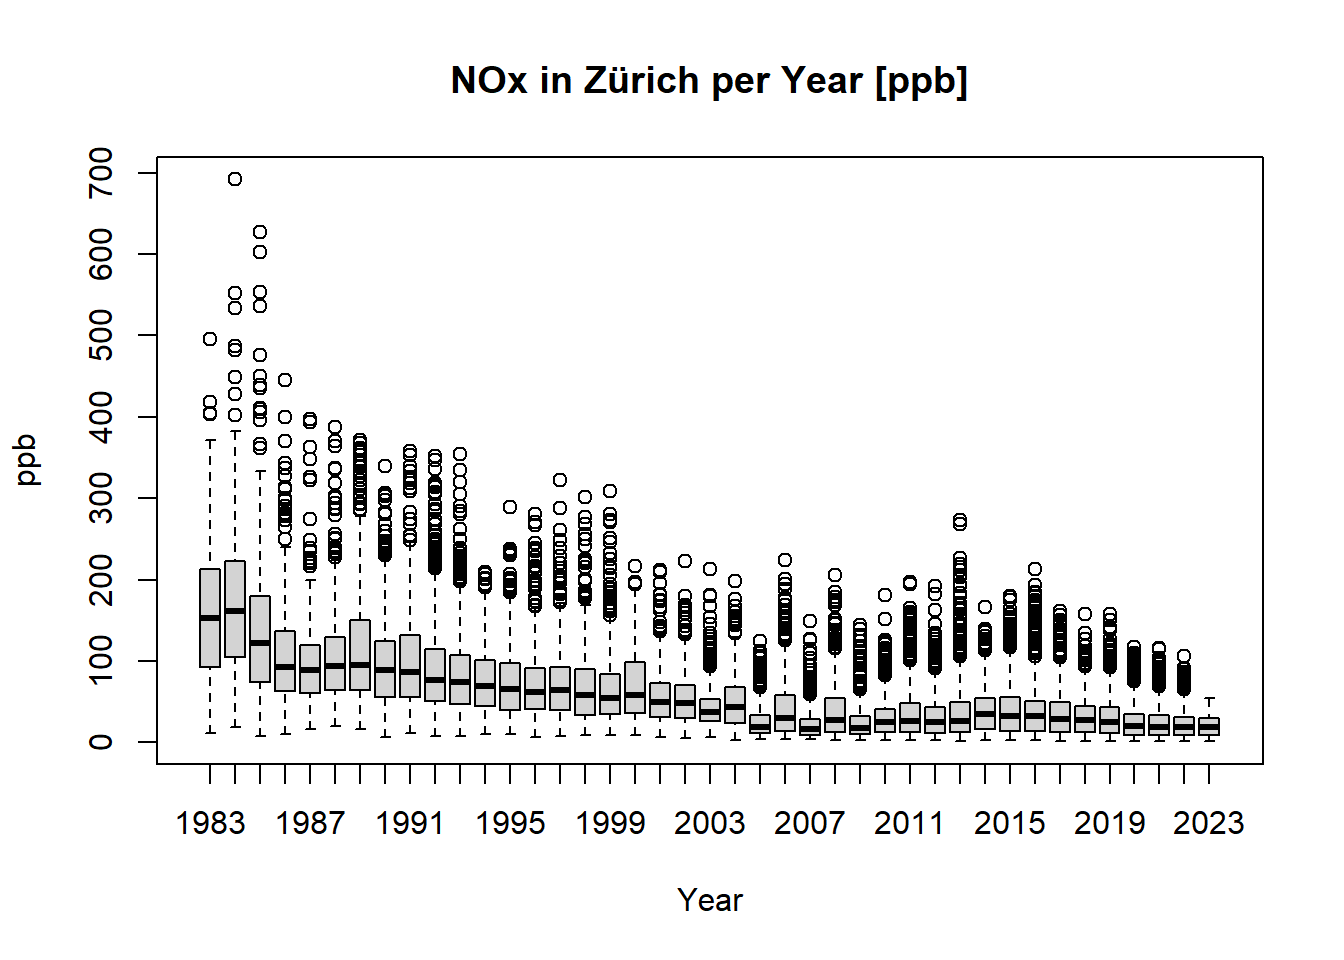
\includegraphics[width=0.45\linewidth]{sustainability_group_files/figure-latex/air.boxplots-2} 

}

\caption{Fig. nnn: CO and NOx per year}\label{fig:air.boxplots}
\end{figure}

~

\hypertarget{difference-of-nitrogen-oxides-per-measuring-station}{%
\subsubsection{Difference of Nitrogen Oxides per measuring
station}\label{difference-of-nitrogen-oxides-per-measuring-station}}

\hfill\break

\begin{figure}

{\centering 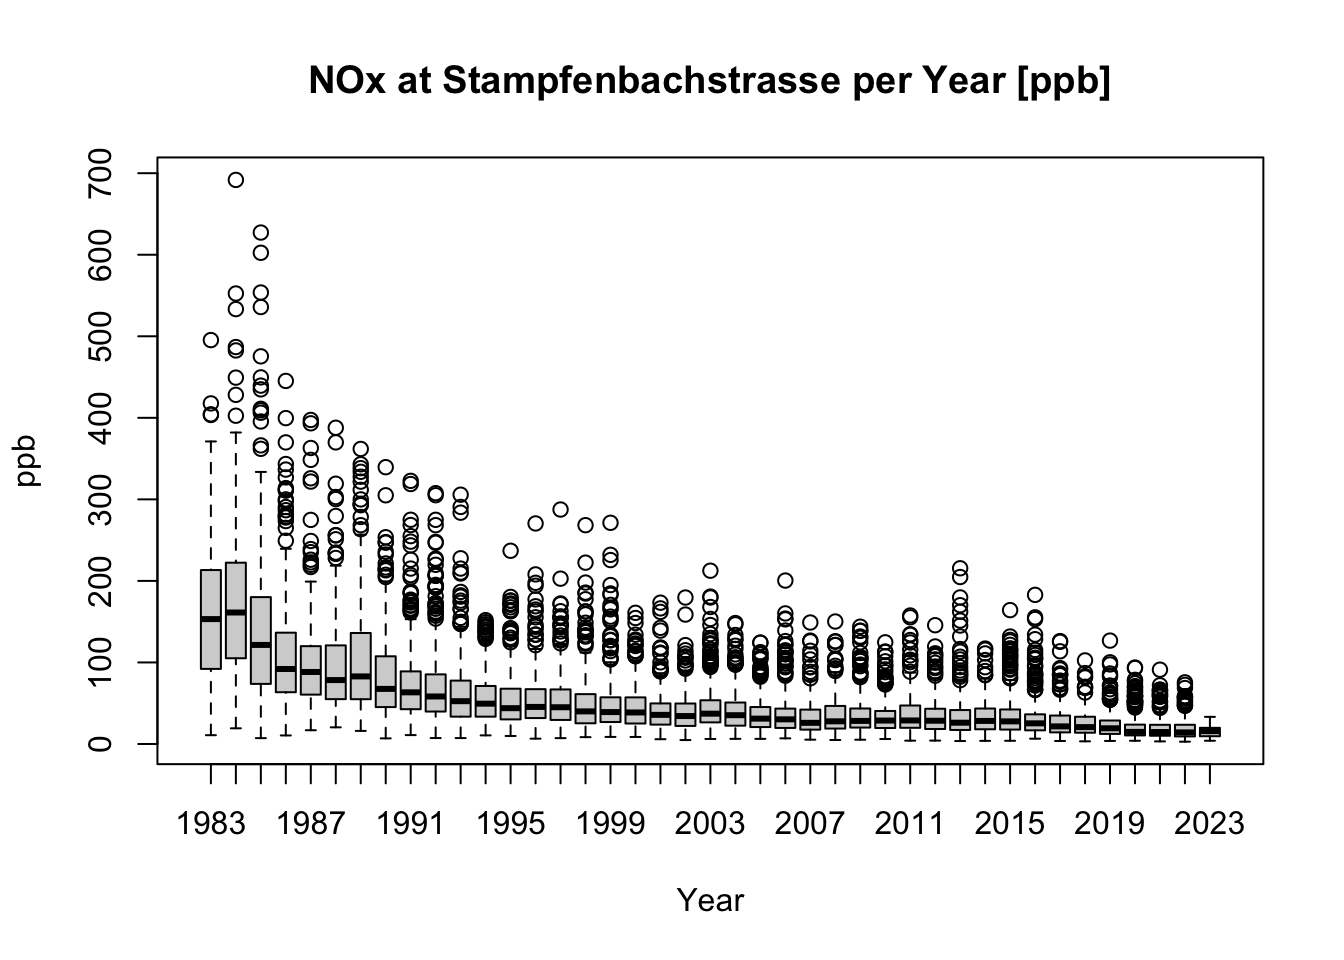
\includegraphics[width=0.33\linewidth]{sustainability_group_files/figure-latex/air.boxplots.station-1} 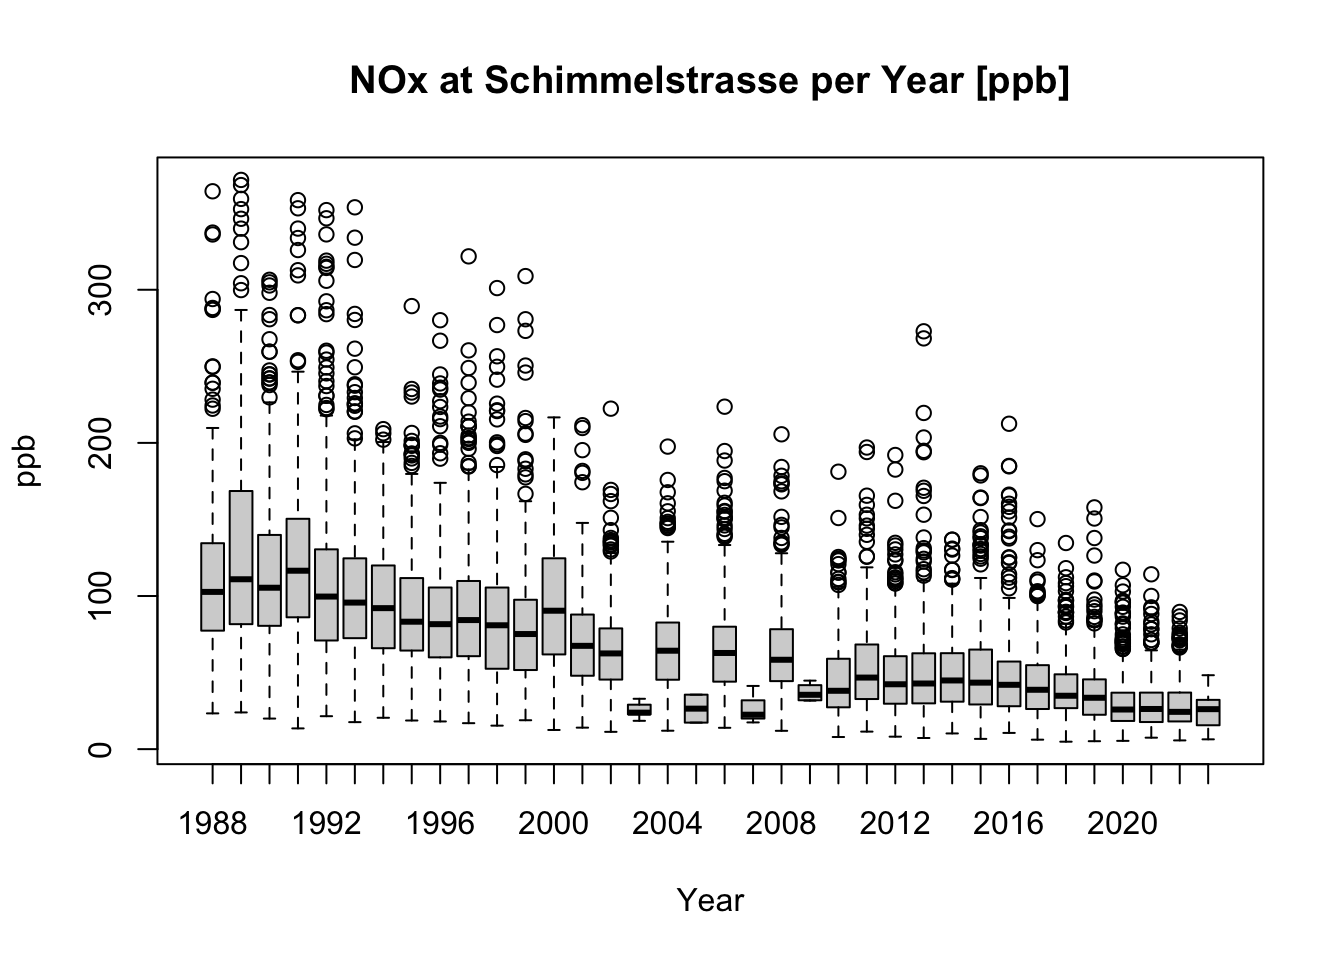
\includegraphics[width=0.33\linewidth]{sustainability_group_files/figure-latex/air.boxplots.station-2} 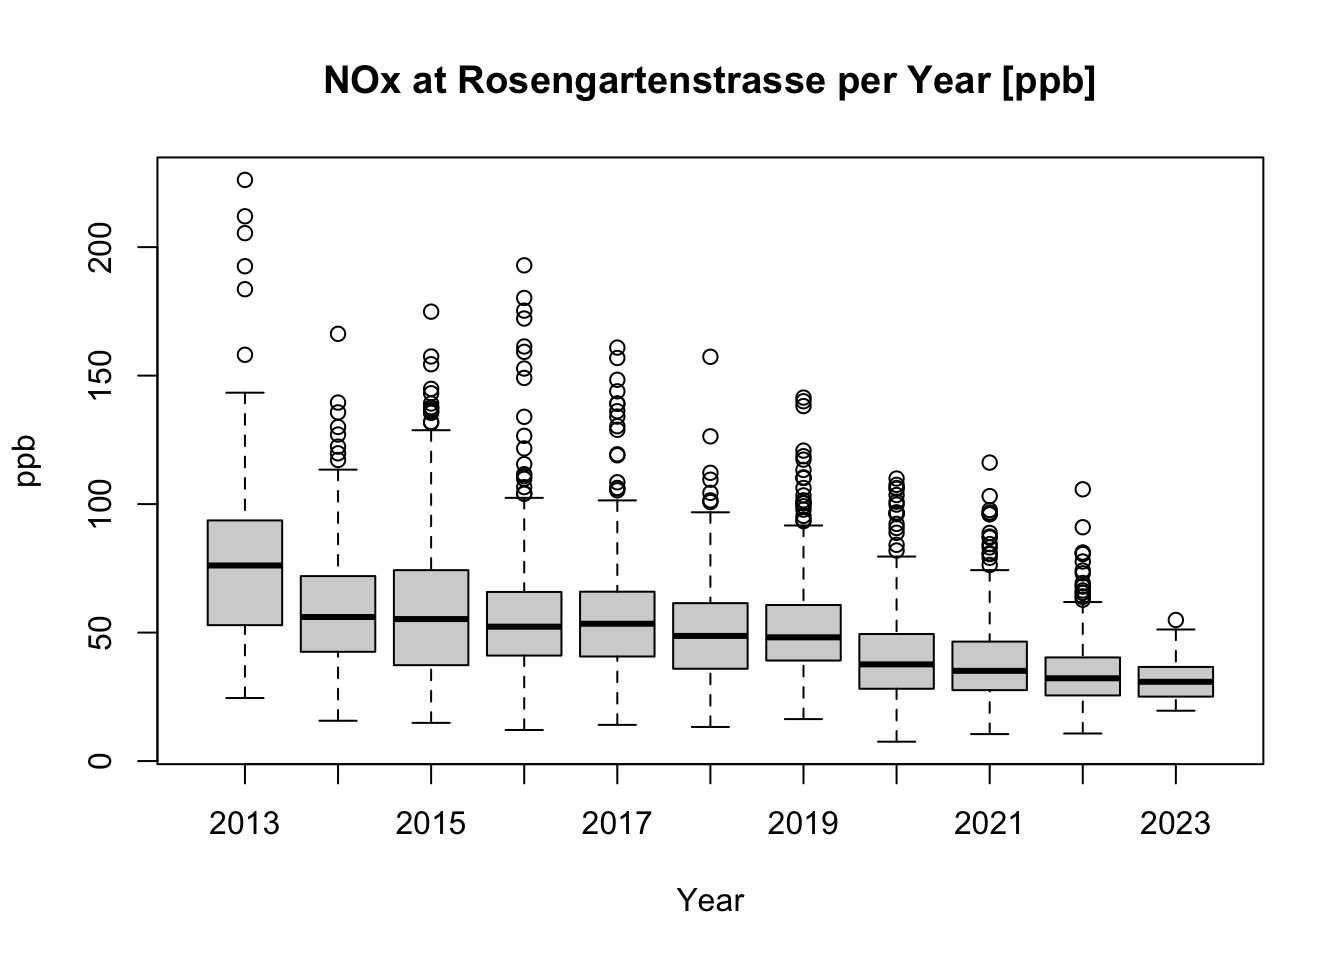
\includegraphics[width=0.33\linewidth]{sustainability_group_files/figure-latex/air.boxplots.station-3} 

}

\caption{Fig. nnn: Nitrogen oxides per monitoring station}\label{fig:air.boxplots.station}
\end{figure}

Nitrogen Oxides have been registered at three different measuring
stations. The values differ as the measuring stations have different
settings, for example main traffic axis, 6 m distance to the street
(Rosengartenstrasse) or moderately frequented road in residential area,
3 m distance to the street (Schimmelstrasse).

Further details on measuring stations:\\
Stampfenbachstrasse:
\url{https://zueriluft.ch/airmo/frontend/station.php?ID=8}\\
Schimmelstrasse:
\url{https://zueriluft.ch/airmo/frontend/station.php?ID=6}\\
Rosengartenstrasse:
\url{https://zueriluft.ch/airmo/frontend/station.php?ID=11}

\hfill\break

The analysis done in the following chapters is based on the measurements
at Stampfenbachstrasse as this data is going back to 1983.

\hfill\break

\hypertarget{temperature-trends}{%
\subsection{Temperature trends}\label{temperature-trends}}

\hfill\break

As a first exploratory data analysis we do not look into the development
of temperature in general as we will have a detailed insight in the
Analysis chapter, we rather look at the evolvement of the maximum and
minimum temperature over time.

\begin{figure}
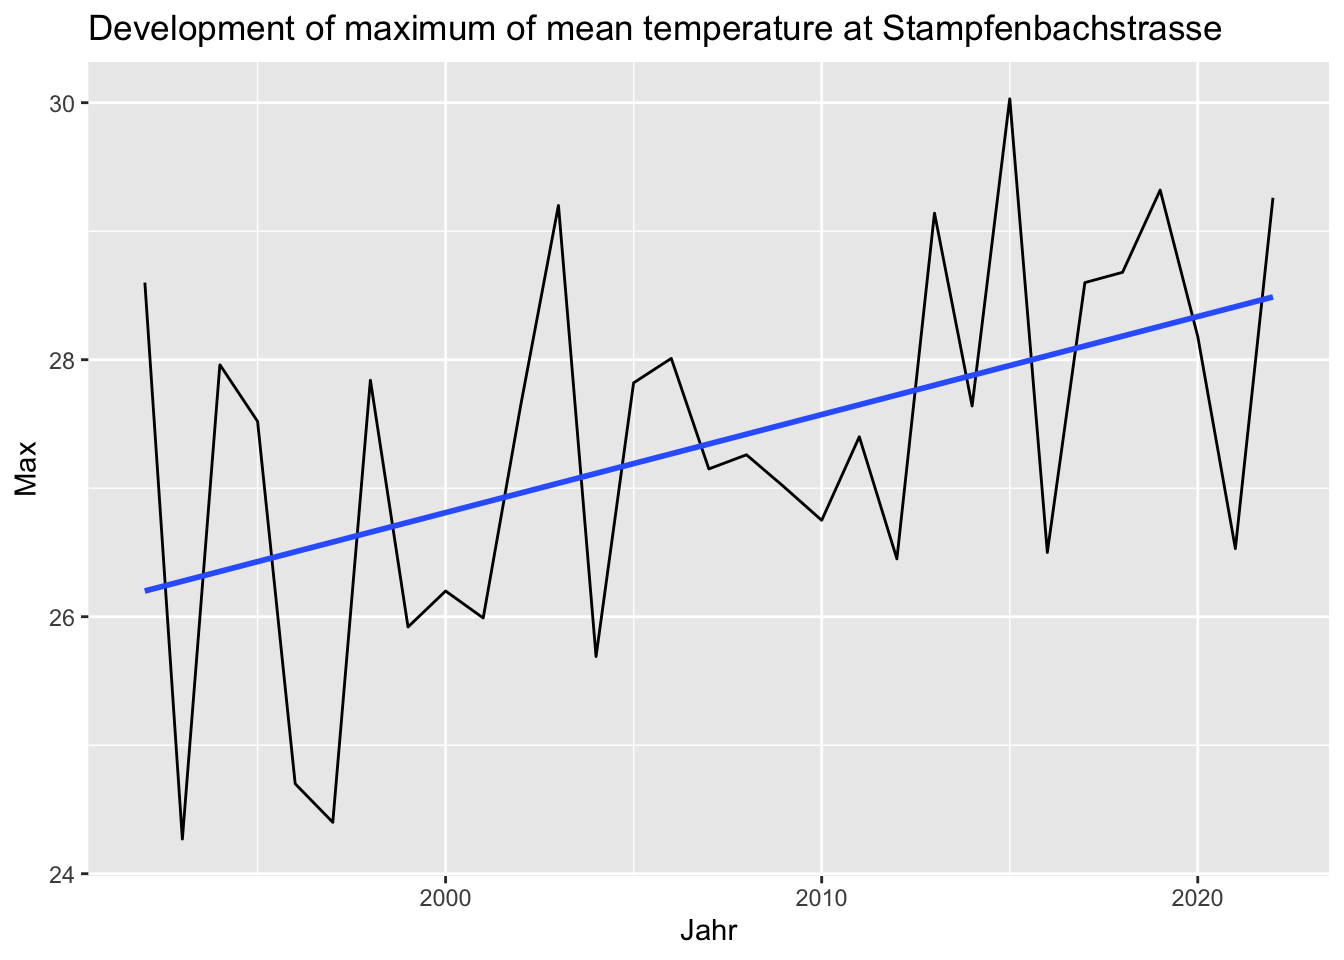
\includegraphics[width=0.33\linewidth]{sustainability_group_files/figure-latex/temperature_trends-1} 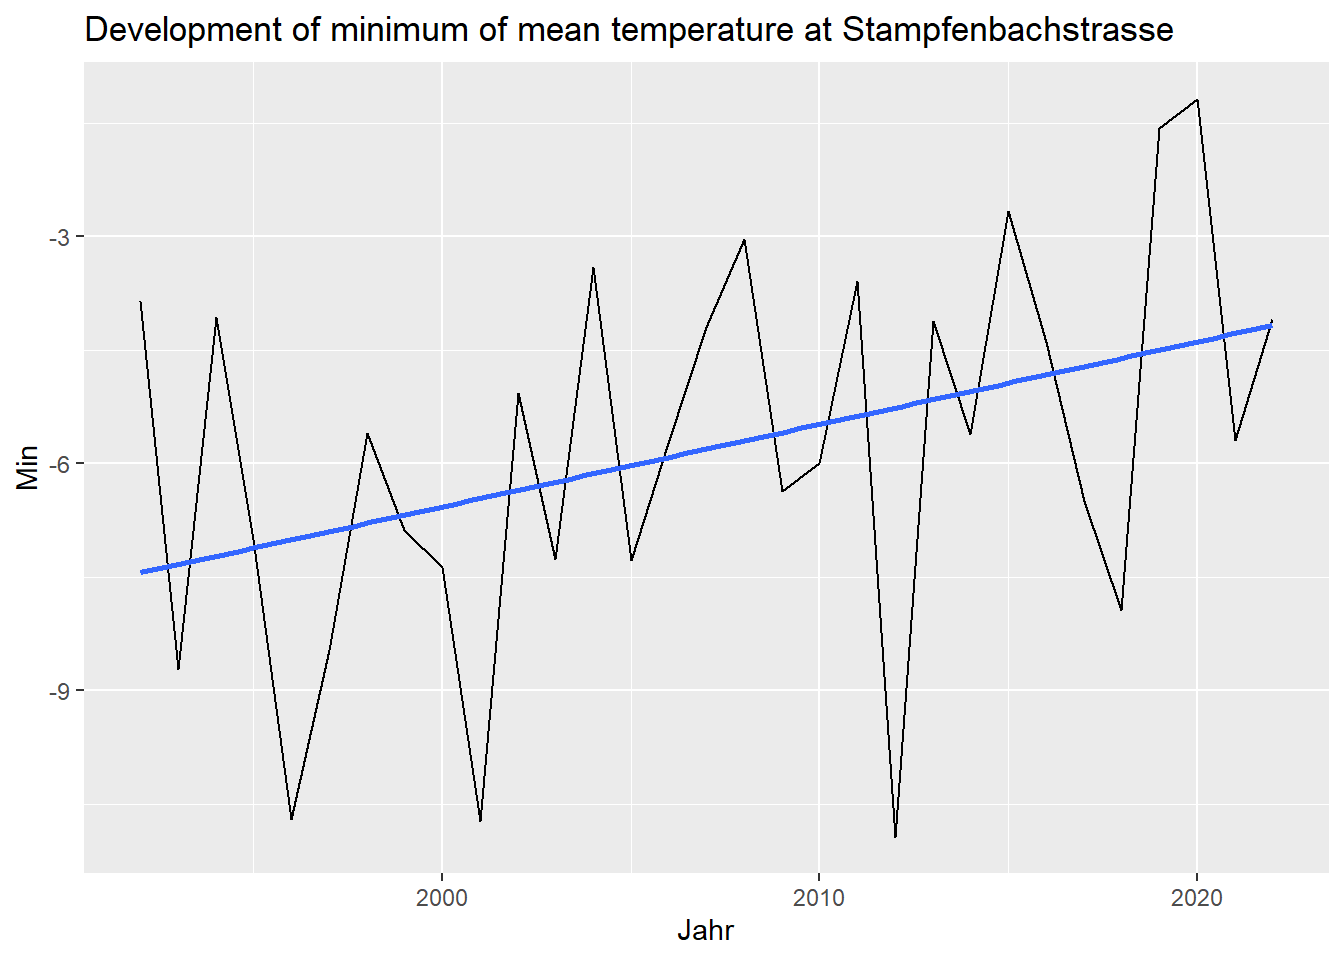
\includegraphics[width=0.33\linewidth]{sustainability_group_files/figure-latex/temperature_trends-2} 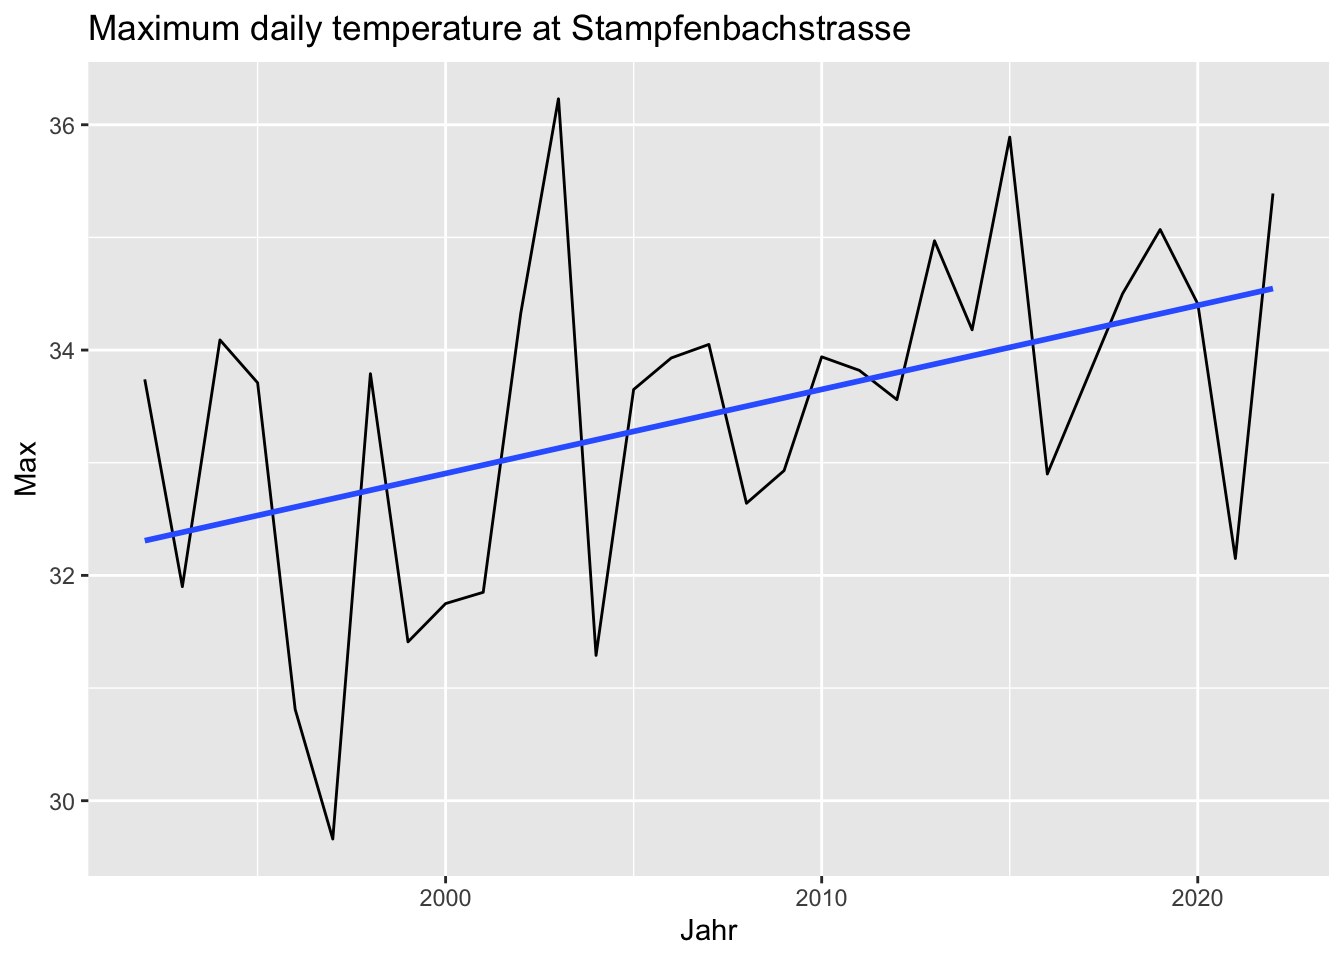
\includegraphics[width=0.33\linewidth]{sustainability_group_files/figure-latex/temperature_trends-3} \caption{Fig. nnn: Temperature trends of maximum and minimum values}\label{fig:temperature_trends}
\end{figure}

The temperatures we have in our data set are daily means. In the left
graph in figure nnn we look at the text text

shows the yearly development of the max of the daily means .

\begin{Shaded}
\begin{Highlighting}[]
\FunctionTok{summary}\NormalTok{(}\FunctionTok{lm}\NormalTok{(meteo.sta}\SpecialCharTok{$}\NormalTok{Max }\SpecialCharTok{\textasciitilde{}}\NormalTok{ meteo.sta}\SpecialCharTok{$}\NormalTok{Jahr))}\SpecialCharTok{$}\NormalTok{coefficients}
\end{Highlighting}
\end{Shaded}

\begin{verbatim}
##                     Estimate  Std. Error   t value    Pr(>|t|)
## (Intercept)    -125.76239113 52.85228101 -2.379507 0.024132656
## meteo.sta$Jahr    0.07628629  0.02633371  2.896906 0.007100222
\end{verbatim}

\begin{Shaded}
\begin{Highlighting}[]
\FunctionTok{summary}\NormalTok{(}\FunctionTok{lm}\NormalTok{(meteo.sta.min}\SpecialCharTok{$}\NormalTok{Min }\SpecialCharTok{\textasciitilde{}}\NormalTok{ meteo.sta.min}\SpecialCharTok{$}\NormalTok{Jahr))}\SpecialCharTok{$}\NormalTok{coefficients}
\end{Highlighting}
\end{Shaded}

\begin{verbatim}
##                        Estimate  Std. Error   t value   Pr(>|t|)
## (Intercept)        -224.4969395 94.83822336 -2.367157 0.02481432
## meteo.sta.min$Jahr    0.1089637  0.04725325  2.305951 0.02845820
\end{verbatim}

\begin{Shaded}
\begin{Highlighting}[]
\FunctionTok{summary}\NormalTok{(}\FunctionTok{lm}\NormalTok{(meteo.sta.max}\SpecialCharTok{$}\NormalTok{Max }\SpecialCharTok{\textasciitilde{}}\NormalTok{ meteo.sta.max}\SpecialCharTok{$}\NormalTok{Jahr))}\SpecialCharTok{$}\NormalTok{coefficients}
\end{Highlighting}
\end{Shaded}

\begin{verbatim}
##                         Estimate  Std. Error   t value   Pr(>|t|)
## (Intercept)        -116.29672177 55.29212464 -2.103314 0.04422930
## meteo.sta.max$Jahr    0.07460081  0.02754937  2.707896 0.01123579
\end{verbatim}

\hfill\break

\hypertarget{trees-in-zuxfcrich-and-their-development-over-the-years}{%
\subsection{Trees in Zürich and their development over the
years}\label{trees-in-zuxfcrich-and-their-development-over-the-years}}

\hfill\break

\begin{figure}
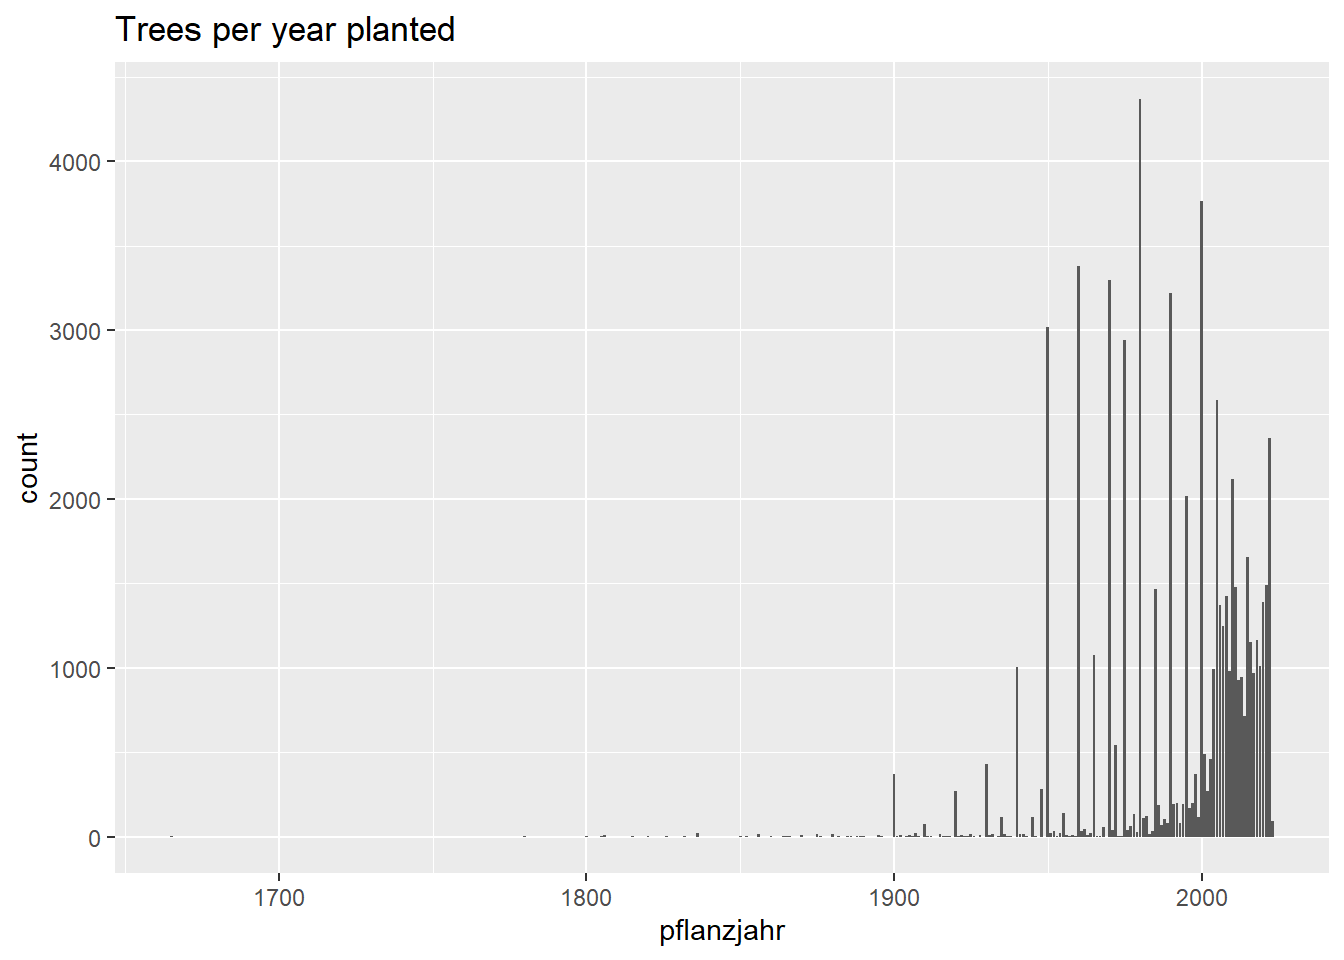
\includegraphics[width=0.33\linewidth]{sustainability_group_files/figure-latex/tree_pflanzjahr-1} 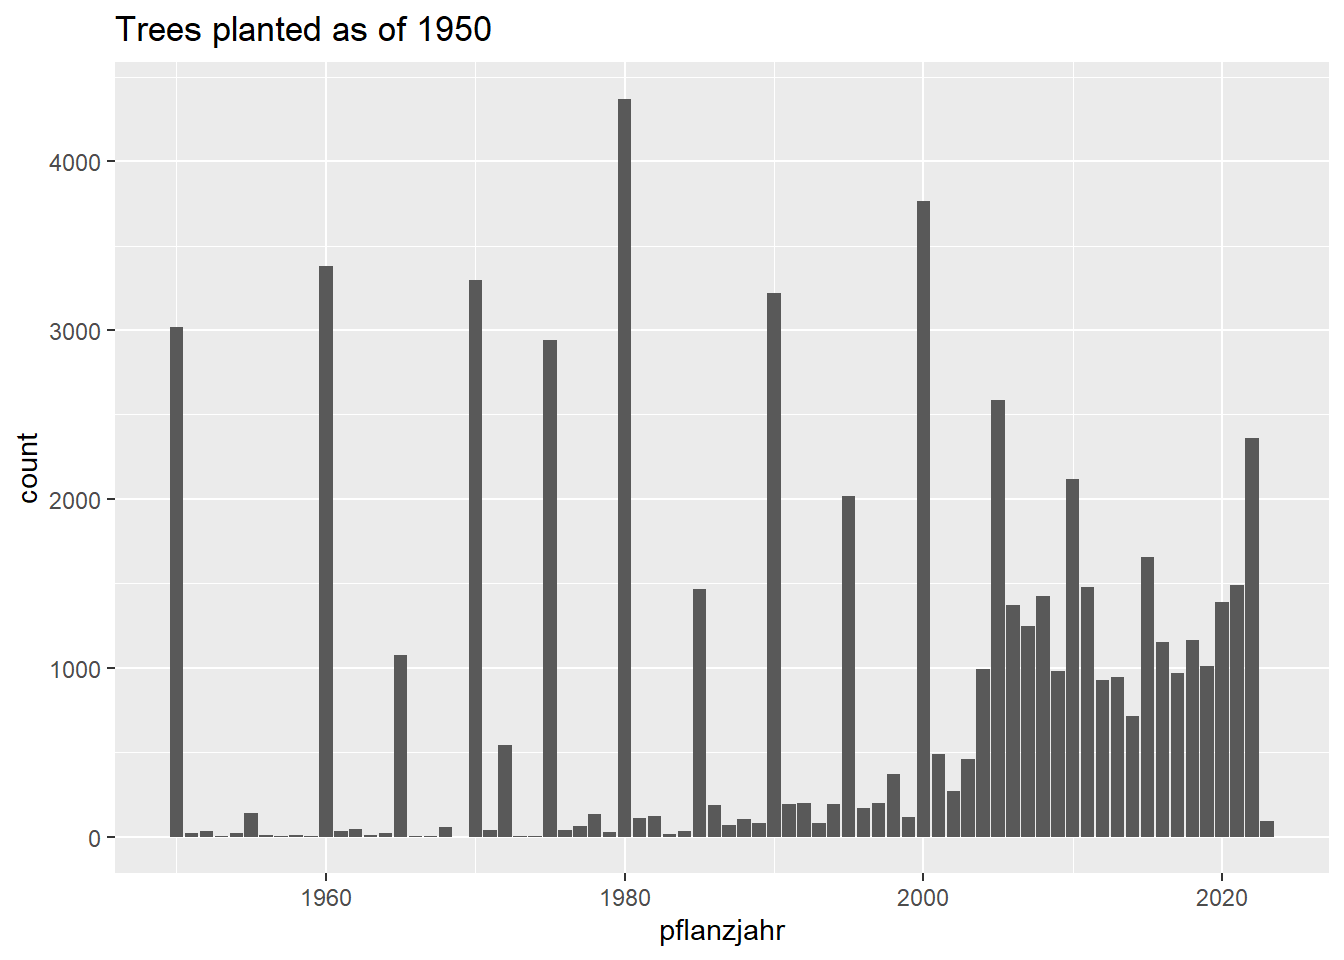
\includegraphics[width=0.33\linewidth]{sustainability_group_files/figure-latex/tree_pflanzjahr-2} 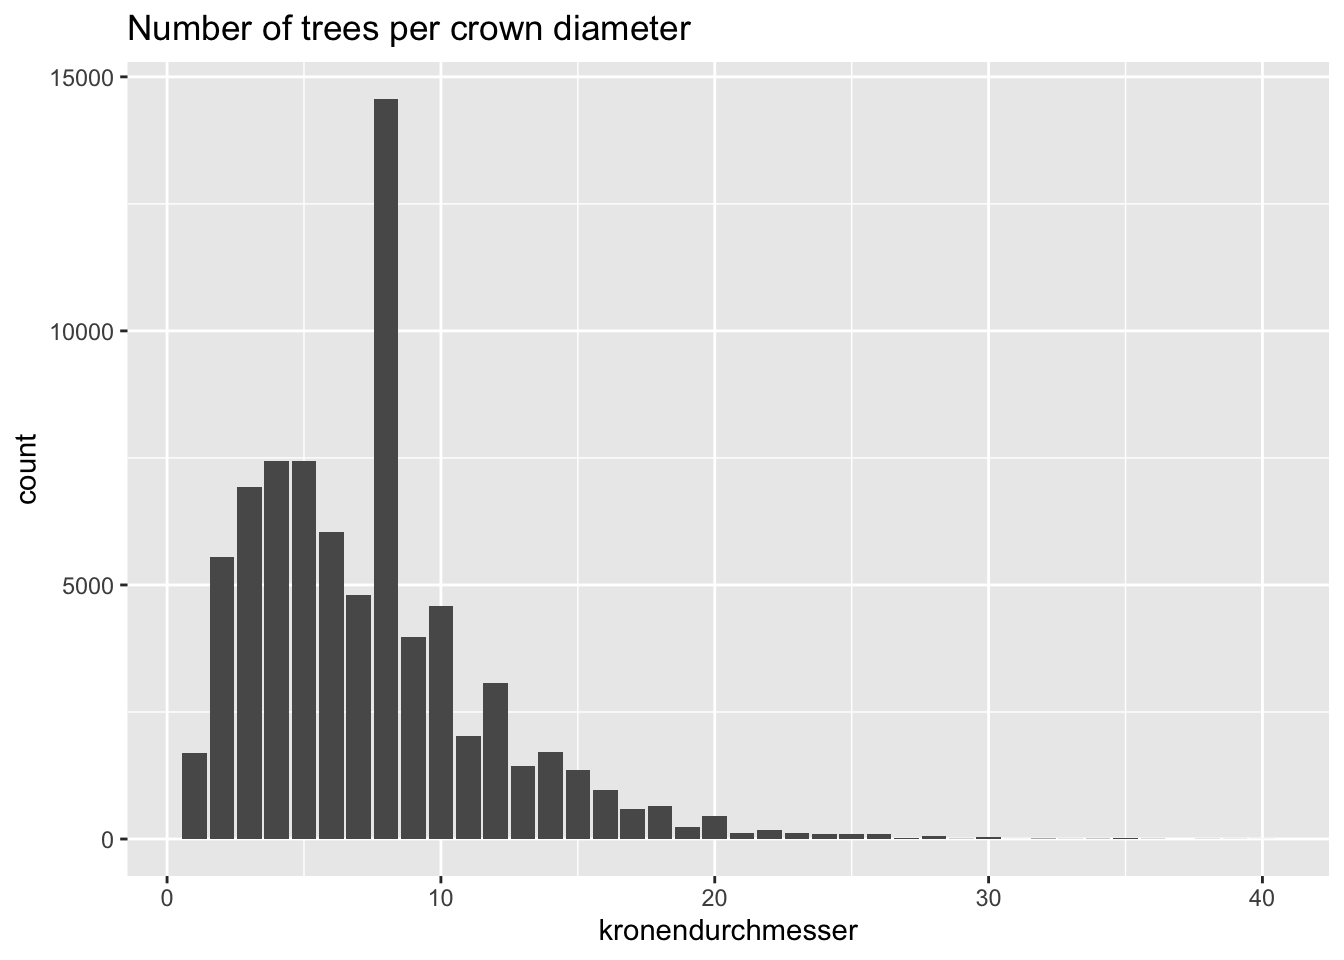
\includegraphics[width=0.33\linewidth]{sustainability_group_files/figure-latex/tree_pflanzjahr-3} \caption{Fig. nnn: Year of planting and crown diameter}\label{fig:tree_pflanzjahr}
\end{figure}

The two graphs in figure nnn on the left side show the numbers of trees
planted per year as of 1950. The graph on the left side reflects our
data on a yearly basis as we get it from our data set. As in earlier
years the number of plantings were mainly summarized every five years,
the middle bar chart shows a more consistent view by grouping 10 years
into one bar.

Planted trees include both, additional trees and replacements. There
were a number of extraordinary environmental influences in recent years,
such as cyclone Lothar in December 1999, or the heavy snow fall in
January 2021 and storm Bernd in July 2021 which damaged more than 2'000
trees on public ground in such a way that they had to be cut down.
Replanting of those 2'000 trees will take time until the year 2025.
\url{https://www.stadt-zuerich.ch/ted/de/index/departement/medien/medienmitteilungen/2021/oktober/211007a.html}

\hfill\break

\hypertarget{remark-on-trees-on-private-ground}{%
\subsection{Remark on trees on private
ground}\label{remark-on-trees-on-private-ground}}

\hfill\break
The City of Zürich is continuously planting trees on public ground as
the awareness that trees are an effective measure to reduce heat in the
city has become a common understanding. But if we broaden our view and
take also the private ground into consideration, we get a different
picture. Half of the area of the tree crowns is on private ground and
those are disappearing in such a pace, that the overall population of
trees is decreasing as well.\\
(\url{https://www.tagesanzeiger.ch/die-stadt-will-ihre-krone-vergroessern-362720147046})

\hfill\break

\hypertarget{analysis}{%
\subsection{Analysis}\label{analysis}}

Having gained an overview of the data, we would now like to analyse the
data in more detail using a few different methodologies.

\hypertarget{timeseries-analysis}{%
\subsubsection{Timeseries Analysis}\label{timeseries-analysis}}

In this section we are trying to see if there is a correlation over time
between the amount of trees and the air quality or temperature. For this
we use timeseries analysis, meaning we need to convert our data into
timeseries objects. After transforming them we can then look at the
decomposition of the objects. Thus we are able to see trends,
seasonality and residuals. However the seasonality is only visible for
air pollution and temperature, as the tree information is only available
on a yearly basis.

\begin{Shaded}
\begin{Highlighting}[]
\NormalTok{meteo }\SpecialCharTok{\%\textless{}\textgreater{}\%} \FunctionTok{complete}\NormalTok{(}\AttributeTok{Date=}\FunctionTok{seq.Date}\NormalTok{(}\FunctionTok{min}\NormalTok{(Date), }\FunctionTok{max}\NormalTok{(Date), }\AttributeTok{by=}\StringTok{\textquotesingle{}day\textquotesingle{}}\NormalTok{))}

\CommentTok{\# Use the time series class of the library stats}
\NormalTok{freq\_daily }\OtherTok{\textless{}{-}} \FloatTok{365.2422}
\NormalTok{temp }\OtherTok{\textless{}{-}}
  \FunctionTok{ts}\NormalTok{(meteo}\SpecialCharTok{$}\NormalTok{T, }\AttributeTok{start=}\FunctionTok{c}\NormalTok{(}\FunctionTok{year}\NormalTok{(}\FunctionTok{min}\NormalTok{(meteo}\SpecialCharTok{$}\NormalTok{Date)),}\FunctionTok{yday}\NormalTok{(}\FunctionTok{min}\NormalTok{(meteo}\SpecialCharTok{$}\NormalTok{Date))),}
     \AttributeTok{frequency=}\NormalTok{freq\_daily) }\SpecialCharTok{\%\textgreater{}\%}
  \FunctionTok{na\_replace}\NormalTok{(}\AttributeTok{fill=}\DecValTok{0}\NormalTok{)}

\CommentTok{\# Stationarity test and decomposition}
\NormalTok{temp\_comp}\OtherTok{=}\FunctionTok{decompose}\NormalTok{(temp)}
\FunctionTok{plot}\NormalTok{(temp\_comp)}
\FunctionTok{title}\NormalTok{(}\AttributeTok{sub =} \StringTok{"Temperature"}\NormalTok{)}

\CommentTok{\# Manual decomposition}
\NormalTok{meteo }\SpecialCharTok{\%\textless{}\textgreater{}\%} \FunctionTok{mutate}\NormalTok{(}\AttributeTok{year=}\FunctionTok{year}\NormalTok{(meteo}\SpecialCharTok{$}\NormalTok{Date)}\SpecialCharTok{+}\FunctionTok{yday}\NormalTok{(meteo}\SpecialCharTok{$}\NormalTok{Date)}\SpecialCharTok{/}\NormalTok{freq\_daily)}
\NormalTok{temp\_trend }\OtherTok{\textless{}{-}} \FunctionTok{lm}\NormalTok{(meteo}\SpecialCharTok{$}\NormalTok{T}\SpecialCharTok{\textasciitilde{}}\NormalTok{meteo}\SpecialCharTok{$}\NormalTok{year)}
\FunctionTok{plot}\NormalTok{(temp, }\AttributeTok{main=}\StringTok{"Temperature trend per year"}\NormalTok{)}
\FunctionTok{abline}\NormalTok{(temp\_trend)}

\CommentTok{\# Prepare yearly data}
\NormalTok{meteo\_yr }\OtherTok{\textless{}{-}}\NormalTok{ meteo }\SpecialCharTok{\%\textgreater{}\%}
  \FunctionTok{mutate}\NormalTok{(}\AttributeTok{temp\_raw=}\FunctionTok{replace\_na}\NormalTok{(T,}\DecValTok{0}\NormalTok{)) }\SpecialCharTok{\%\textgreater{}\%}
  \FunctionTok{group\_by}\NormalTok{(}\AttributeTok{Year=}\FunctionTok{year}\NormalTok{(Date)) }\SpecialCharTok{\%\textgreater{}\%}
  \FunctionTok{filter}\NormalTok{(Year}\SpecialCharTok{\textgreater{}=}\DecValTok{1980} \SpecialCharTok{\&}\NormalTok{ Year}\SpecialCharTok{\textless{}=}\DecValTok{2021}\NormalTok{) }\SpecialCharTok{\%\textgreater{}\%}
  \FunctionTok{summarize}\NormalTok{(}\AttributeTok{temp=}\FunctionTok{mean}\NormalTok{(temp\_raw)) }\SpecialCharTok{\%\textgreater{}\%}
  \FunctionTok{ungroup}\NormalTok{()}

\NormalTok{temp\_yr }\OtherTok{\textless{}{-}} \FunctionTok{ts}\NormalTok{(temp, }\AttributeTok{start=}\FunctionTok{min}\NormalTok{(meteo\_yr}\SpecialCharTok{$}\NormalTok{Year))}
\NormalTok{tb\_temp\_ts }\OtherTok{\textless{}{-}} \FunctionTok{tbats}\NormalTok{(temp\_yr)}

\CommentTok{\# Differ}
\DocumentationTok{\#\# twice{-}difference the CO2 data}
\NormalTok{temp\_d2 }\OtherTok{\textless{}{-}} \FunctionTok{diff}\NormalTok{(temp, }\AttributeTok{differences =} \DecValTok{1}\NormalTok{)}

\DocumentationTok{\#\# difference the differenced CO2 data}
\NormalTok{temp\_d2d12 }\OtherTok{\textless{}{-}} \FunctionTok{diff}\NormalTok{(temp\_d2, }\AttributeTok{lag =} \DecValTok{12}\NormalTok{)}
\DocumentationTok{\#\# plot the newly differenced data}
\FunctionTok{plot}\NormalTok{(temp\_d2d12, }\AttributeTok{ylab =} \StringTok{"Temperature without trend and seasonality"}\NormalTok{)}
\end{Highlighting}
\end{Shaded}

\begin{figure}
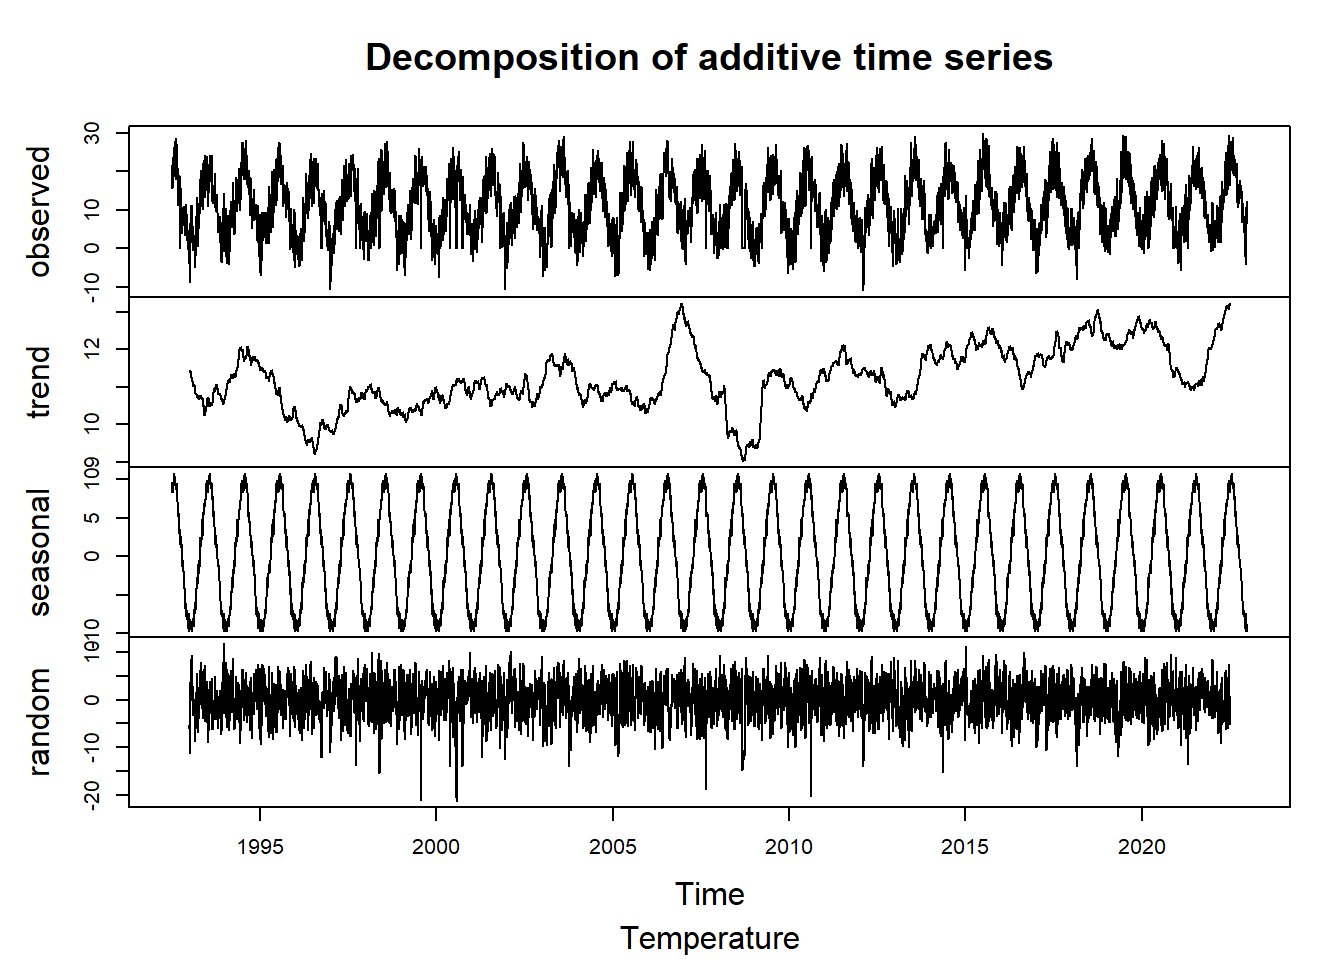
\includegraphics[width=0.33\linewidth]{sustainability_group_files/figure-latex/time_meteo-1} 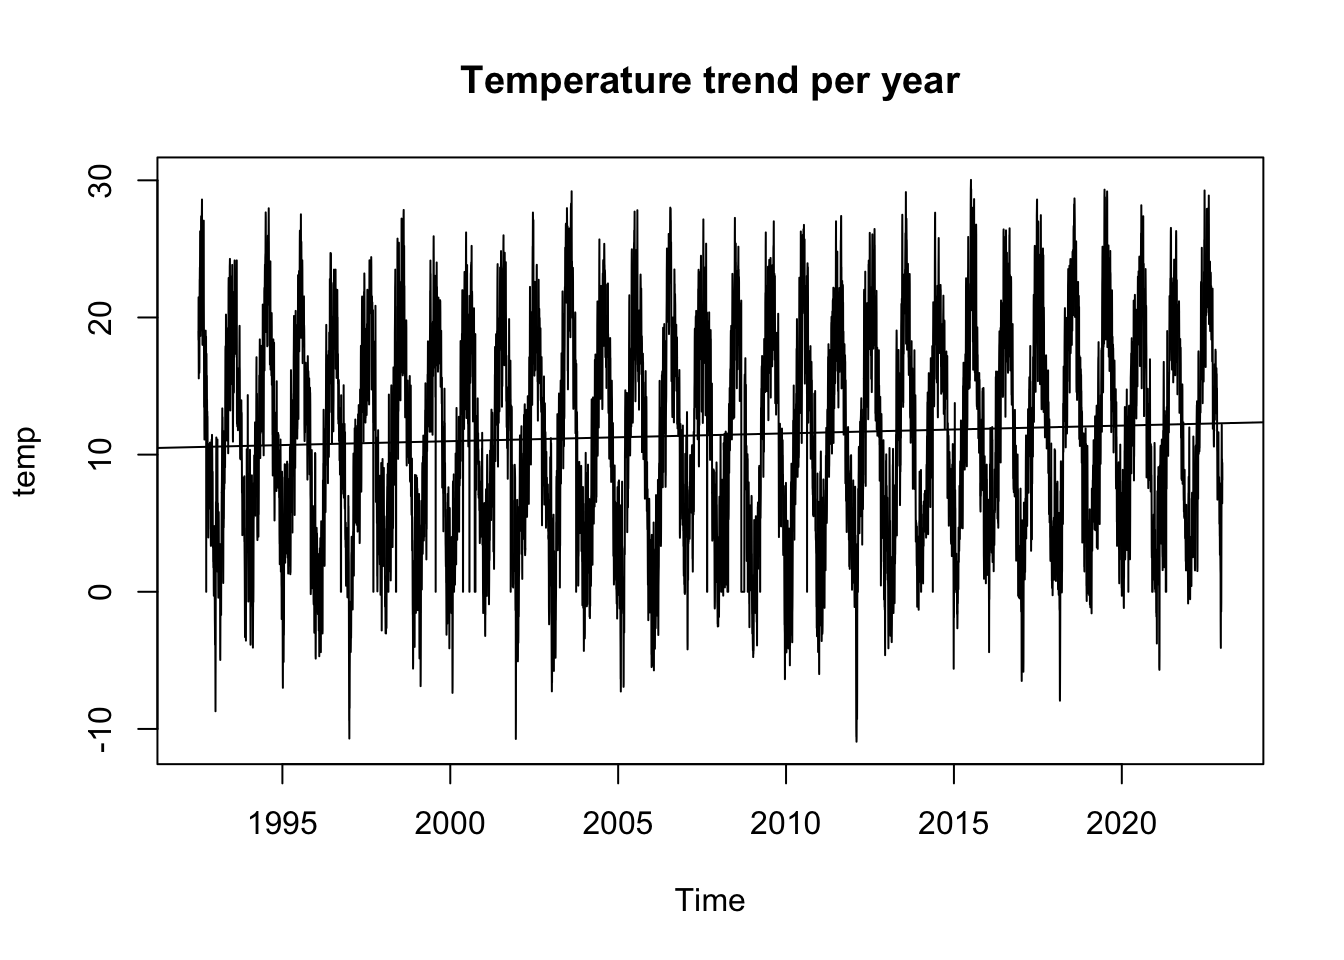
\includegraphics[width=0.33\linewidth]{sustainability_group_files/figure-latex/time_meteo-2} 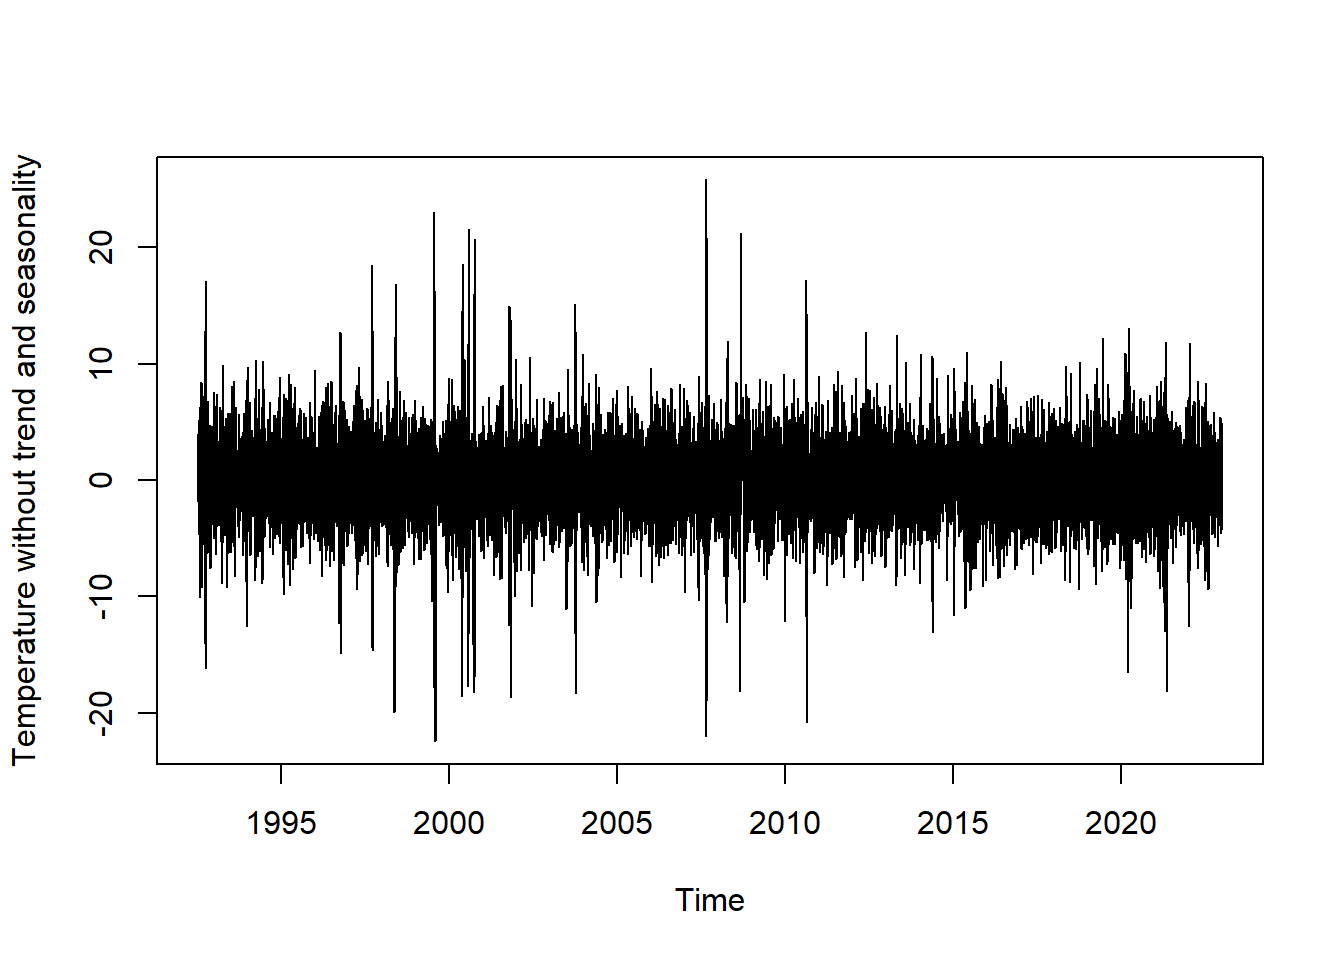
\includegraphics[width=0.33\linewidth]{sustainability_group_files/figure-latex/time_meteo-3} \caption{Fig. nnn: Temperature timeseries}\label{fig:time_meteo}
\end{figure}

Generally we can see that the temperature is slightly rising over time.
There is a slight upwards trend noticeable and it is also important to
remember how much danger a temperature increase of just one percent can
be for the biodiversity.

\begin{Shaded}
\begin{Highlighting}[]
\NormalTok{air.short }\SpecialCharTok{\%\textless{}\textgreater{}\%} \FunctionTok{complete}\NormalTok{(}\AttributeTok{Date=}\FunctionTok{seq.Date}\NormalTok{(}\FunctionTok{min}\NormalTok{(Date), }\FunctionTok{max}\NormalTok{(Date), }\AttributeTok{by=}\StringTok{\textquotesingle{}day\textquotesingle{}}\NormalTok{))}

\CommentTok{\# Use the time series class of the library stats}
\NormalTok{freq\_daily }\OtherTok{\textless{}{-}} \FloatTok{365.2422}
\NormalTok{co }\OtherTok{\textless{}{-}}
  \FunctionTok{ts}\NormalTok{(air.short}\SpecialCharTok{$}\NormalTok{CO, }\AttributeTok{start=}\FunctionTok{c}\NormalTok{(}\FunctionTok{year}\NormalTok{(}\FunctionTok{min}\NormalTok{(air.short}\SpecialCharTok{$}\NormalTok{Date)),}\FunctionTok{yday}\NormalTok{(}\FunctionTok{min}\NormalTok{(air.short}\SpecialCharTok{$}\NormalTok{Date))),}
     \AttributeTok{frequency=}\NormalTok{freq\_daily) }\SpecialCharTok{\%\textgreater{}\%}
  \FunctionTok{na\_replace}\NormalTok{(}\AttributeTok{fill=}\DecValTok{0}\NormalTok{)}
\NormalTok{NOx }\OtherTok{\textless{}{-}}
  \FunctionTok{ts}\NormalTok{(air.short}\SpecialCharTok{$}\NormalTok{NOx, }\AttributeTok{start=}\FunctionTok{c}\NormalTok{(}\FunctionTok{year}\NormalTok{(}\FunctionTok{min}\NormalTok{(air.short}\SpecialCharTok{$}\NormalTok{Date)), }\FunctionTok{yday}\NormalTok{(}\FunctionTok{min}\NormalTok{(air.short}\SpecialCharTok{$}\NormalTok{Date))),}
     \AttributeTok{frequency=}\NormalTok{freq\_daily) }\SpecialCharTok{\%\textgreater{}\%}
  \FunctionTok{na\_replace}\NormalTok{(}\AttributeTok{fill=}\DecValTok{0}\NormalTok{)}

\CommentTok{\# Stationarity test and decomposition}
\CommentTok{\# adf.test(co,k=0)}
\CommentTok{\# adf.test(NOx,k=0)}
\NormalTok{co\_comp}\OtherTok{=}\FunctionTok{decompose}\NormalTok{(co)}
\NormalTok{NOx\_comp}\OtherTok{=}\FunctionTok{decompose}\NormalTok{(NOx)}

\CommentTok{\# Manual decomposition}
\NormalTok{air.short }\SpecialCharTok{\%\textless{}\textgreater{}\%} \FunctionTok{mutate}\NormalTok{(}\AttributeTok{year=}\FunctionTok{year}\NormalTok{(air.short}\SpecialCharTok{$}\NormalTok{Date)}\SpecialCharTok{+}\FunctionTok{yday}\NormalTok{(air.short}\SpecialCharTok{$}\NormalTok{Date)}\SpecialCharTok{/}\NormalTok{freq\_daily)}
\NormalTok{co\_trend }\OtherTok{\textless{}{-}} \FunctionTok{lm}\NormalTok{(air.short}\SpecialCharTok{$}\NormalTok{CO}\SpecialCharTok{\textasciitilde{}}\NormalTok{air.short}\SpecialCharTok{$}\NormalTok{year)}
\NormalTok{NOx\_trend }\OtherTok{\textless{}{-}} \FunctionTok{lm}\NormalTok{(air.short}\SpecialCharTok{$}\NormalTok{NOx}\SpecialCharTok{\textasciitilde{}}\NormalTok{air.short}\SpecialCharTok{$}\NormalTok{year)}

\NormalTok{air\_yr }\OtherTok{\textless{}{-}}\NormalTok{ air.short }\SpecialCharTok{\%\textgreater{}\%}
  \FunctionTok{mutate}\NormalTok{(}\AttributeTok{co\_raw=}\FunctionTok{replace\_na}\NormalTok{(CO,}\DecValTok{0}\NormalTok{), }\AttributeTok{NOx\_raw=}\FunctionTok{replace\_na}\NormalTok{(NOx,}\DecValTok{0}\NormalTok{)) }\SpecialCharTok{\%\textgreater{}\%}
  \FunctionTok{group\_by}\NormalTok{(}\AttributeTok{Year=}\FunctionTok{year}\NormalTok{(Date)) }\SpecialCharTok{\%\textgreater{}\%}
  \FunctionTok{filter}\NormalTok{(Year}\SpecialCharTok{\textgreater{}=}\DecValTok{1980} \SpecialCharTok{\&}\NormalTok{ Year}\SpecialCharTok{\textless{}=}\DecValTok{2021}\NormalTok{) }\SpecialCharTok{\%\textgreater{}\%}
  \FunctionTok{summarize}\NormalTok{(}\AttributeTok{co=}\FunctionTok{sum}\NormalTok{(co\_raw), }\AttributeTok{NOx=}\FunctionTok{mean}\NormalTok{(NOx\_raw)) }\SpecialCharTok{\%\textgreater{}\%}
  \FunctionTok{ungroup}\NormalTok{()}

\CommentTok{\# Time series}
\NormalTok{co\_yr }\OtherTok{\textless{}{-}} \FunctionTok{ts}\NormalTok{(air\_yr}\SpecialCharTok{$}\NormalTok{co, }\AttributeTok{start=}\FunctionTok{min}\NormalTok{(air\_yr}\SpecialCharTok{$}\NormalTok{Year), }\AttributeTok{frequency=}\DecValTok{1}\NormalTok{)}
\NormalTok{NOx\_yr }\OtherTok{\textless{}{-}} \FunctionTok{ts}\NormalTok{(air\_yr}\SpecialCharTok{$}\NormalTok{NOx, }\AttributeTok{start=}\FunctionTok{min}\NormalTok{(air\_yr}\SpecialCharTok{$}\NormalTok{Year), }\AttributeTok{frequency=}\DecValTok{1}\NormalTok{)}

\CommentTok{\# plot(co\_yr)}
\CommentTok{\# plot(NOx\_yr)}

\CommentTok{\# Manual decomposition}
\NormalTok{co\_yr\_trend }\OtherTok{\textless{}{-}} \FunctionTok{lm}\NormalTok{(air\_yr}\SpecialCharTok{$}\NormalTok{co}\SpecialCharTok{\textasciitilde{}}\NormalTok{air\_yr}\SpecialCharTok{$}\NormalTok{Year)}
\FunctionTok{plot}\NormalTok{(co\_yr, }\AttributeTok{xlab=}\StringTok{\textquotesingle{}Year\textquotesingle{}}\NormalTok{, }\AttributeTok{ylab=}\StringTok{\textquotesingle{}Average co pollution\textquotesingle{}}\NormalTok{)}
\FunctionTok{abline}\NormalTok{(co\_yr\_trend)}
\FunctionTok{title}\NormalTok{(}\AttributeTok{main =} \StringTok{"CO development over the years and trend line"}\NormalTok{)}
\NormalTok{NOx\_yr\_trend }\OtherTok{\textless{}{-}} \FunctionTok{lm}\NormalTok{(air\_yr}\SpecialCharTok{$}\NormalTok{NOx}\SpecialCharTok{\textasciitilde{}}\NormalTok{air\_yr}\SpecialCharTok{$}\NormalTok{Year)}
\FunctionTok{plot}\NormalTok{(NOx\_yr, }\AttributeTok{xlab=}\StringTok{\textquotesingle{}Year\textquotesingle{}}\NormalTok{, }\AttributeTok{ylab=}\StringTok{\textquotesingle{}Average NOx pollution\textquotesingle{}}\NormalTok{)}
\FunctionTok{abline}\NormalTok{(NOx\_yr\_trend)}
\FunctionTok{title}\NormalTok{(}\AttributeTok{main =} \StringTok{"NOx development over the years and trend line"}\NormalTok{)}

\NormalTok{tree\_ts }\OtherTok{\textless{}{-}}  \FunctionTok{ts}\NormalTok{(tree\_ts\_sum}\SpecialCharTok{$}\NormalTok{sum\_trees, }\AttributeTok{start=}\FunctionTok{min}\NormalTok{(tree\_ts\_sum}\SpecialCharTok{$}\NormalTok{pflanzjahr), }\AttributeTok{frequency=}\DecValTok{1}\NormalTok{)}
\NormalTok{tb\_tree\_ts }\OtherTok{\textless{}{-}} \FunctionTok{tbats}\NormalTok{(tree\_ts)}
\NormalTok{tb\_co\_ts }\OtherTok{\textless{}{-}} \FunctionTok{tbats}\NormalTok{(co\_yr)}
\NormalTok{tb\_nox\_ts }\OtherTok{\textless{}{-}} \FunctionTok{tbats}\NormalTok{(NOx\_yr)}

\FunctionTok{plot}\NormalTok{(}\FunctionTok{residuals}\NormalTok{(tb\_co\_ts))}
\FunctionTok{title}\NormalTok{(}\AttributeTok{main =} \StringTok{"Residuals of CO"}\NormalTok{)}
\FunctionTok{plot}\NormalTok{(}\FunctionTok{residuals}\NormalTok{(tb\_nox\_ts))}
\FunctionTok{title}\NormalTok{(}\AttributeTok{main =} \StringTok{"Residuals of NOx"}\NormalTok{)}

\CommentTok{\# "Forecast"}
\CommentTok{\# plot(forecast(co\_yr))}
\end{Highlighting}
\end{Shaded}

\begin{figure}
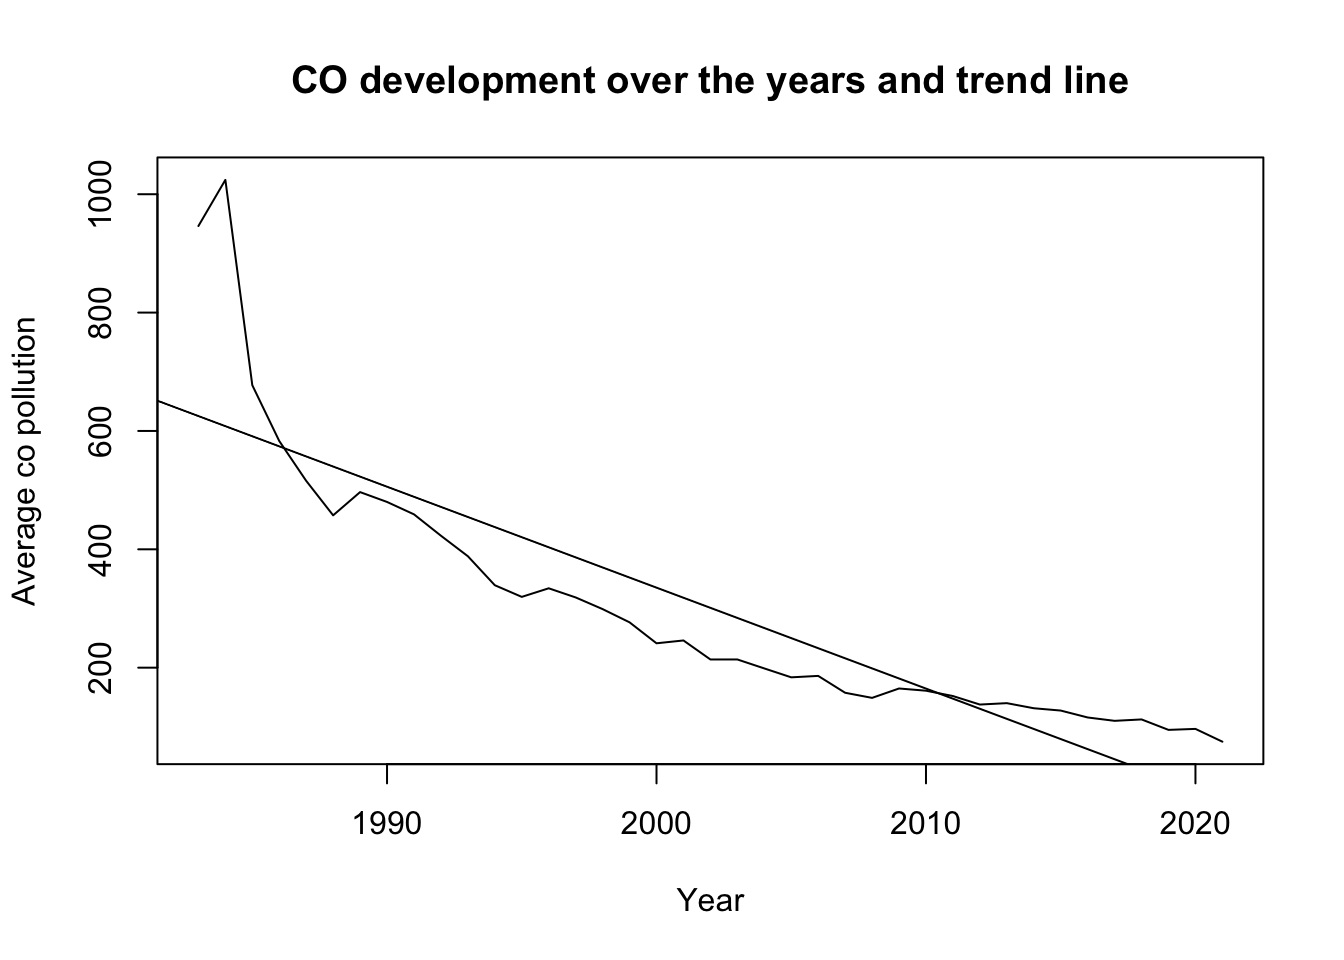
\includegraphics[width=0.5\linewidth]{sustainability_group_files/figure-latex/time_air-1} 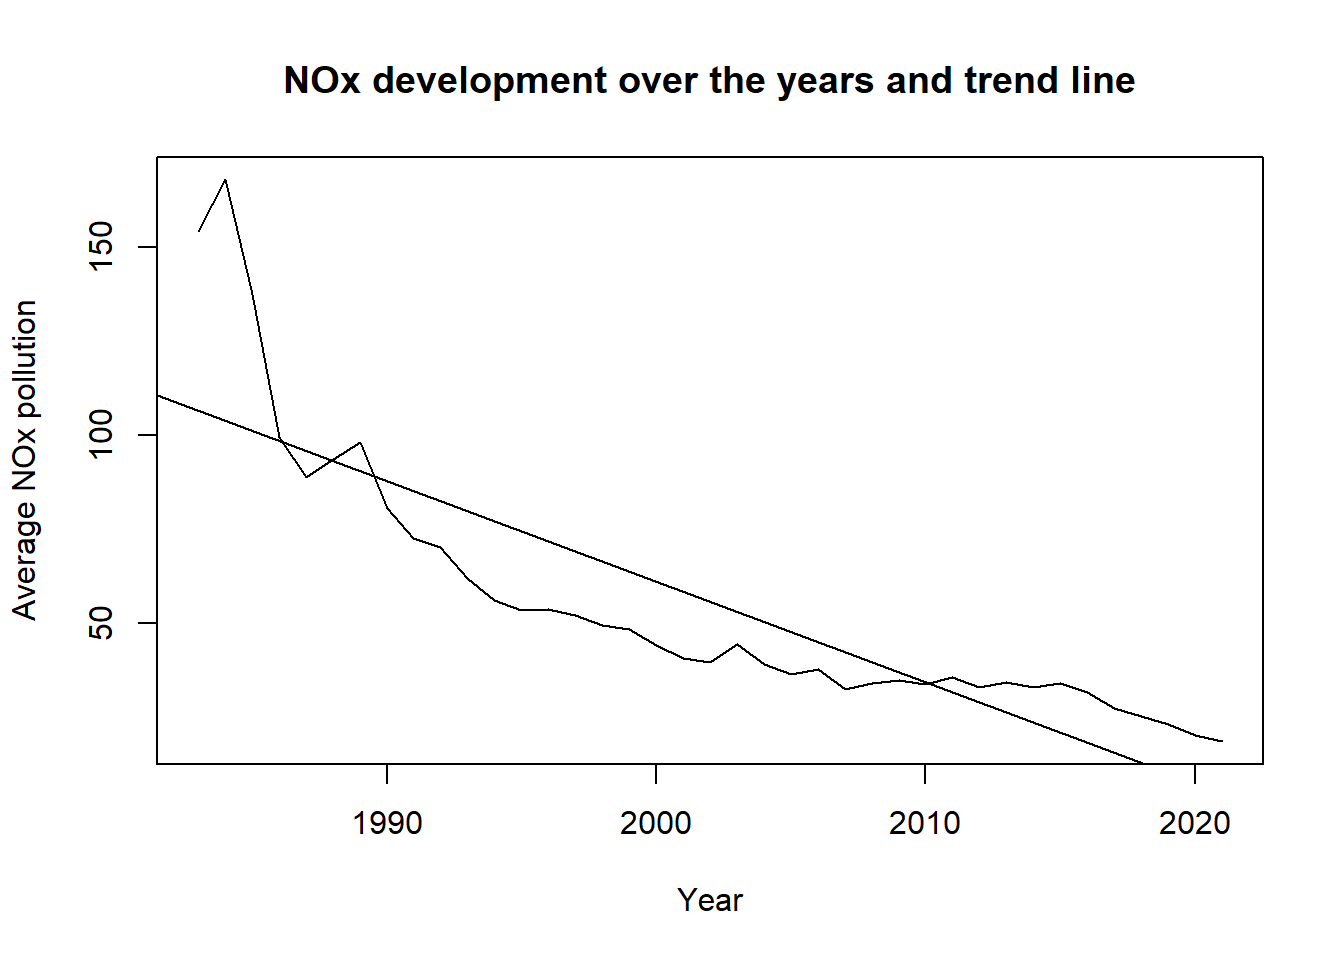
\includegraphics[width=0.5\linewidth]{sustainability_group_files/figure-latex/time_air-2} 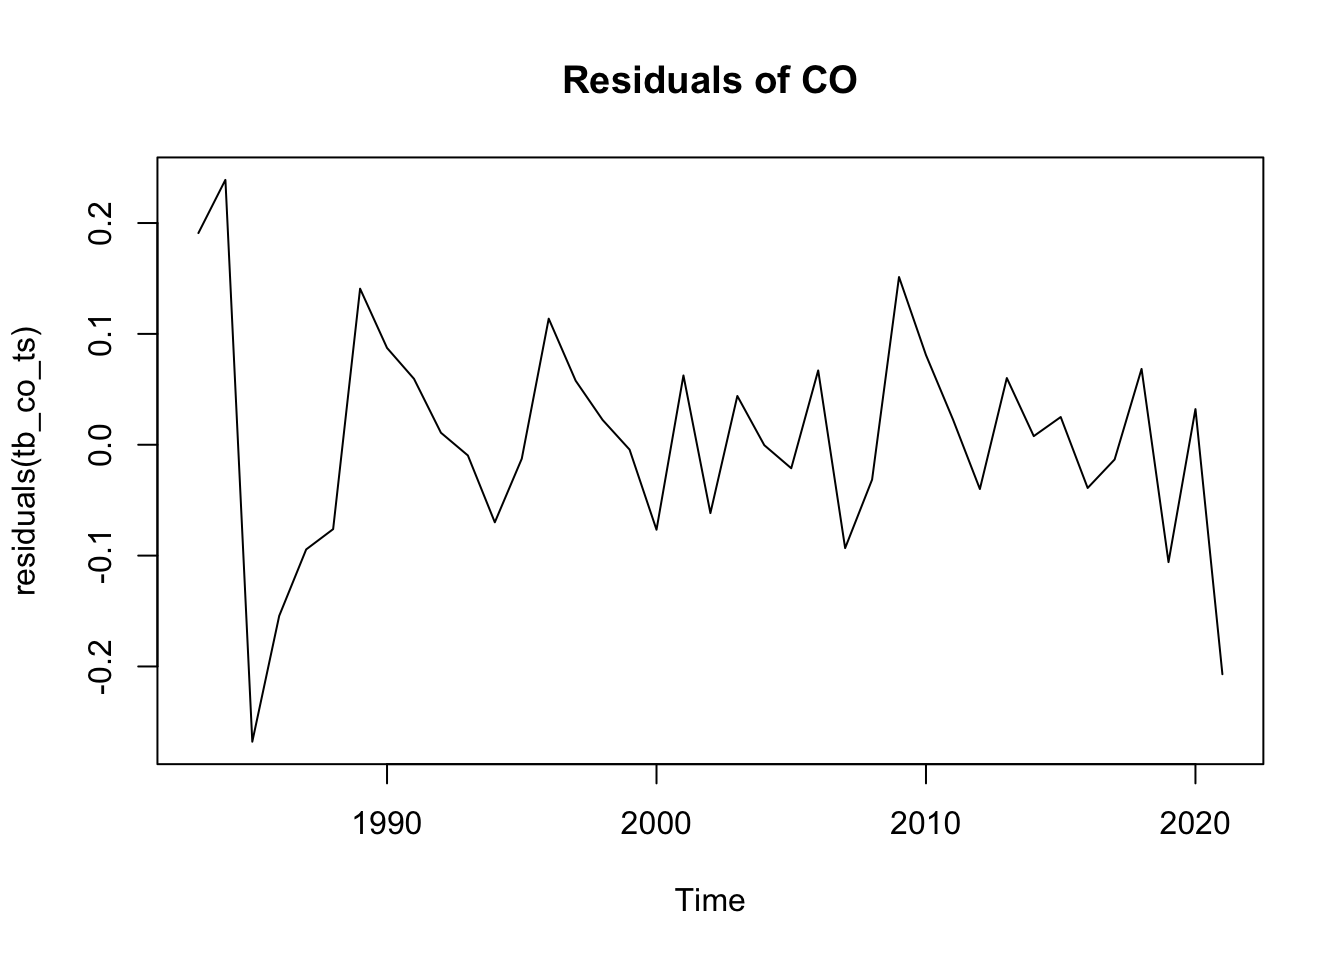
\includegraphics[width=0.5\linewidth]{sustainability_group_files/figure-latex/time_air-3} 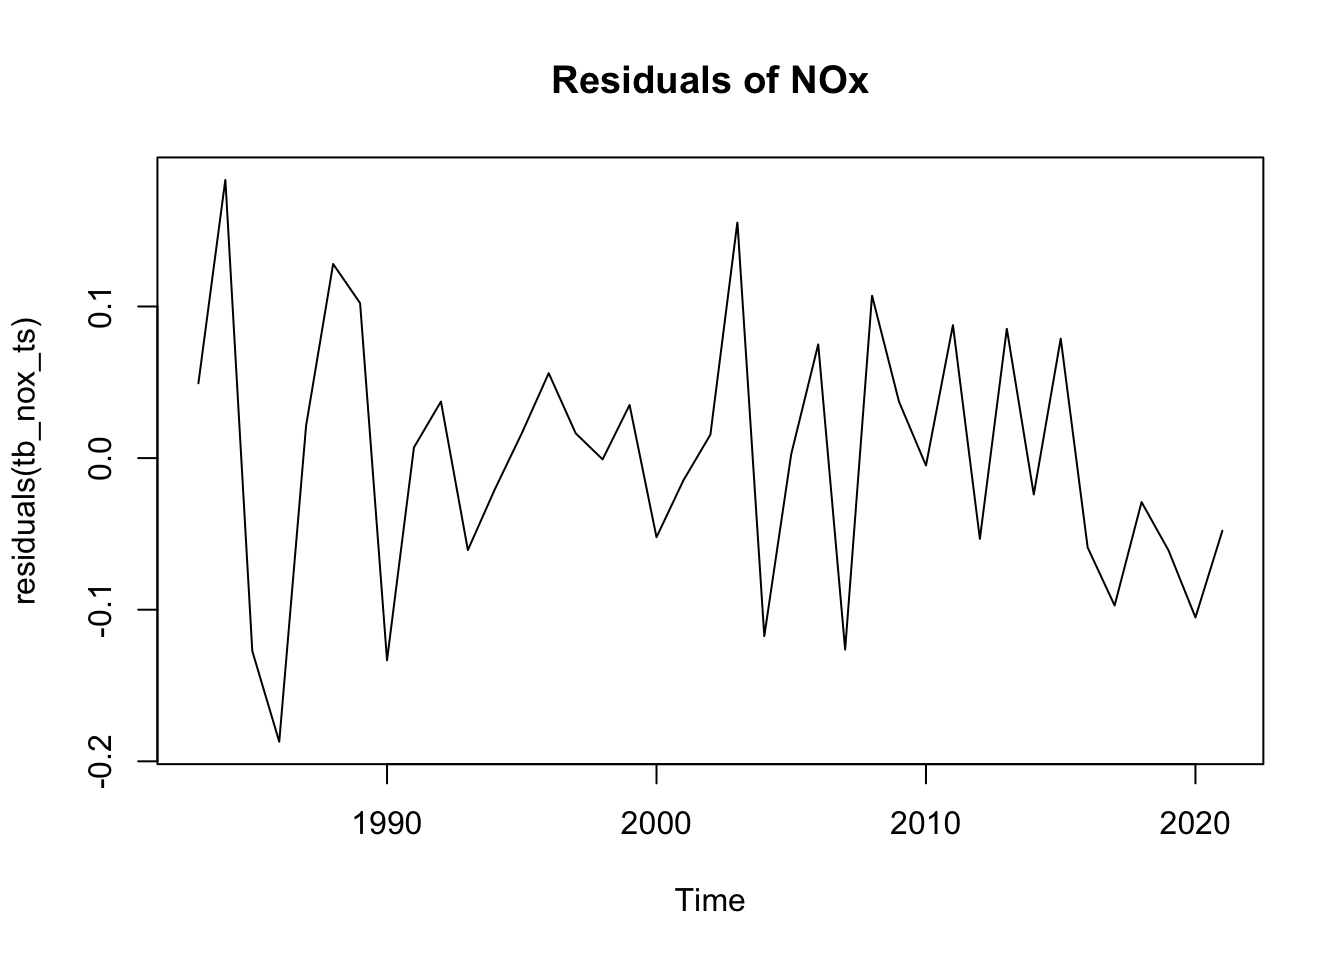
\includegraphics[width=0.5\linewidth]{sustainability_group_files/figure-latex/time_air-4} \caption{Fig. nnn: Air Quality timeseries}\label{fig:time_air}
\end{figure}

The timeseries analysis of Carbon monoxide (co) and Nitrogen oxide (NOx)
show that the they are closely correlated. It is further clear that they
have both decreased drastically since the 1980 in Zürich. It is unlikely
that the whole change can be attributed to the growing number of trees
and green spaces in Zürich. It is more likely that a variety of factors
including advancement in technologies and changes in laws and
regulations contributed as well to the improvement in air quality.

\begin{Shaded}
\begin{Highlighting}[]
\CommentTok{\# Make the time series comparable}
\NormalTok{temp\_comp\_random }\OtherTok{\textless{}{-}} \FunctionTok{data.frame}\NormalTok{(}\AttributeTok{Date=}\FunctionTok{time}\NormalTok{(temp\_comp}\SpecialCharTok{$}\NormalTok{random), }\AttributeTok{Random=}\NormalTok{temp\_comp}\SpecialCharTok{$}\NormalTok{random)}
\NormalTok{co\_comp\_random }\OtherTok{\textless{}{-}} \FunctionTok{data.frame}\NormalTok{(}\AttributeTok{Date=}\FunctionTok{time}\NormalTok{(co\_comp}\SpecialCharTok{$}\NormalTok{random), }\AttributeTok{Random=}\NormalTok{co\_comp}\SpecialCharTok{$}\NormalTok{random)}
\NormalTok{NOx\_comp\_random }\OtherTok{\textless{}{-}} \FunctionTok{data.frame}\NormalTok{(}\AttributeTok{Date=}\FunctionTok{time}\NormalTok{(NOx\_comp}\SpecialCharTok{$}\NormalTok{random), }\AttributeTok{Random=}\NormalTok{NOx\_comp}\SpecialCharTok{$}\NormalTok{random)}

\NormalTok{window }\OtherTok{\textless{}{-}} \FunctionTok{list}\NormalTok{(}\AttributeTok{start=}\DecValTok{1980}\NormalTok{,}\AttributeTok{end=}\DecValTok{2021}\NormalTok{)}

\NormalTok{temp\_comp\_random }\SpecialCharTok{\%\textless{}\textgreater{}\%} \FunctionTok{filter}\NormalTok{(Date}\SpecialCharTok{\textgreater{}=}\NormalTok{window}\SpecialCharTok{$}\NormalTok{start}\SpecialCharTok{\&}\NormalTok{Date}\SpecialCharTok{\textless{}}\NormalTok{window}\SpecialCharTok{$}\NormalTok{end)}
\NormalTok{co\_comp\_random }\SpecialCharTok{\%\textless{}\textgreater{}\%} \FunctionTok{filter}\NormalTok{(Date}\SpecialCharTok{\textgreater{}=}\NormalTok{window}\SpecialCharTok{$}\NormalTok{start}\SpecialCharTok{\&}\NormalTok{Date}\SpecialCharTok{\textless{}}\NormalTok{window}\SpecialCharTok{$}\NormalTok{end)}
\NormalTok{NOx\_comp\_random }\SpecialCharTok{\%\textless{}\textgreater{}\%} \FunctionTok{filter}\NormalTok{(Date}\SpecialCharTok{\textgreater{}=}\NormalTok{window}\SpecialCharTok{$}\NormalTok{start}\SpecialCharTok{\&}\NormalTok{Date}\SpecialCharTok{\textless{}}\NormalTok{window}\SpecialCharTok{$}\NormalTok{end)}

\NormalTok{temp\_comp\_random\_ts }\OtherTok{\textless{}{-}} \FunctionTok{ts}\NormalTok{(temp\_comp\_random}\SpecialCharTok{$}\NormalTok{Random, }\AttributeTok{start=}\FunctionTok{c}\NormalTok{(window}\SpecialCharTok{$}\NormalTok{start,}\DecValTok{1}\NormalTok{), }\AttributeTok{frequency=}\NormalTok{freq\_daily)}
\NormalTok{co\_comp\_random\_ts }\OtherTok{\textless{}{-}} \FunctionTok{ts}\NormalTok{(co\_comp\_random}\SpecialCharTok{$}\NormalTok{Random, }\AttributeTok{start=}\FunctionTok{c}\NormalTok{(window}\SpecialCharTok{$}\NormalTok{start,}\DecValTok{1}\NormalTok{), }\AttributeTok{frequency=}\NormalTok{freq\_daily)}
\NormalTok{NOx\_comp\_random\_ts }\OtherTok{\textless{}{-}} \FunctionTok{ts}\NormalTok{(NOx\_comp\_random}\SpecialCharTok{$}\NormalTok{Random, }\AttributeTok{start=}\FunctionTok{c}\NormalTok{(window}\SpecialCharTok{$}\NormalTok{start,}\DecValTok{1}\NormalTok{), }\AttributeTok{frequency=}\NormalTok{freq\_daily)}


\CommentTok{\# Cross correlation function}
\FunctionTok{ccf}\NormalTok{(}\FunctionTok{residuals}\NormalTok{(tb\_tree\_ts), }\FunctionTok{residuals}\NormalTok{(tb\_nox\_ts), }
    \AttributeTok{lag.max =} \DecValTok{300}\NormalTok{,}
    \AttributeTok{main =} \StringTok{"Trees {-} NOx Cross{-}Correlation Plot"}\NormalTok{,}
    \AttributeTok{ylab =} \StringTok{"CCF"}\NormalTok{)}
\FunctionTok{ccf}\NormalTok{(}\FunctionTok{residuals}\NormalTok{(tb\_tree\_ts), }\FunctionTok{residuals}\NormalTok{(tb\_co\_ts), }
    \AttributeTok{lag.max =} \DecValTok{300}\NormalTok{,}
    \AttributeTok{main =} \StringTok{"Trees {-} CO Cross{-}Correlation Plot"}\NormalTok{,}
    \AttributeTok{ylab =} \StringTok{"CCF"}\NormalTok{)}
\FunctionTok{ccf}\NormalTok{(}\FunctionTok{residuals}\NormalTok{(tb\_tree\_ts), }\FunctionTok{residuals}\NormalTok{(tb\_temp\_ts), }
    \AttributeTok{lag.max =} \DecValTok{300}\NormalTok{,}
    \AttributeTok{main =} \StringTok{"Trees {-} Temperature Cross{-}Correlation Plot"}\NormalTok{,}
    \AttributeTok{ylab =} \StringTok{"CCF"}\NormalTok{)}
\end{Highlighting}
\end{Shaded}

\begin{figure}
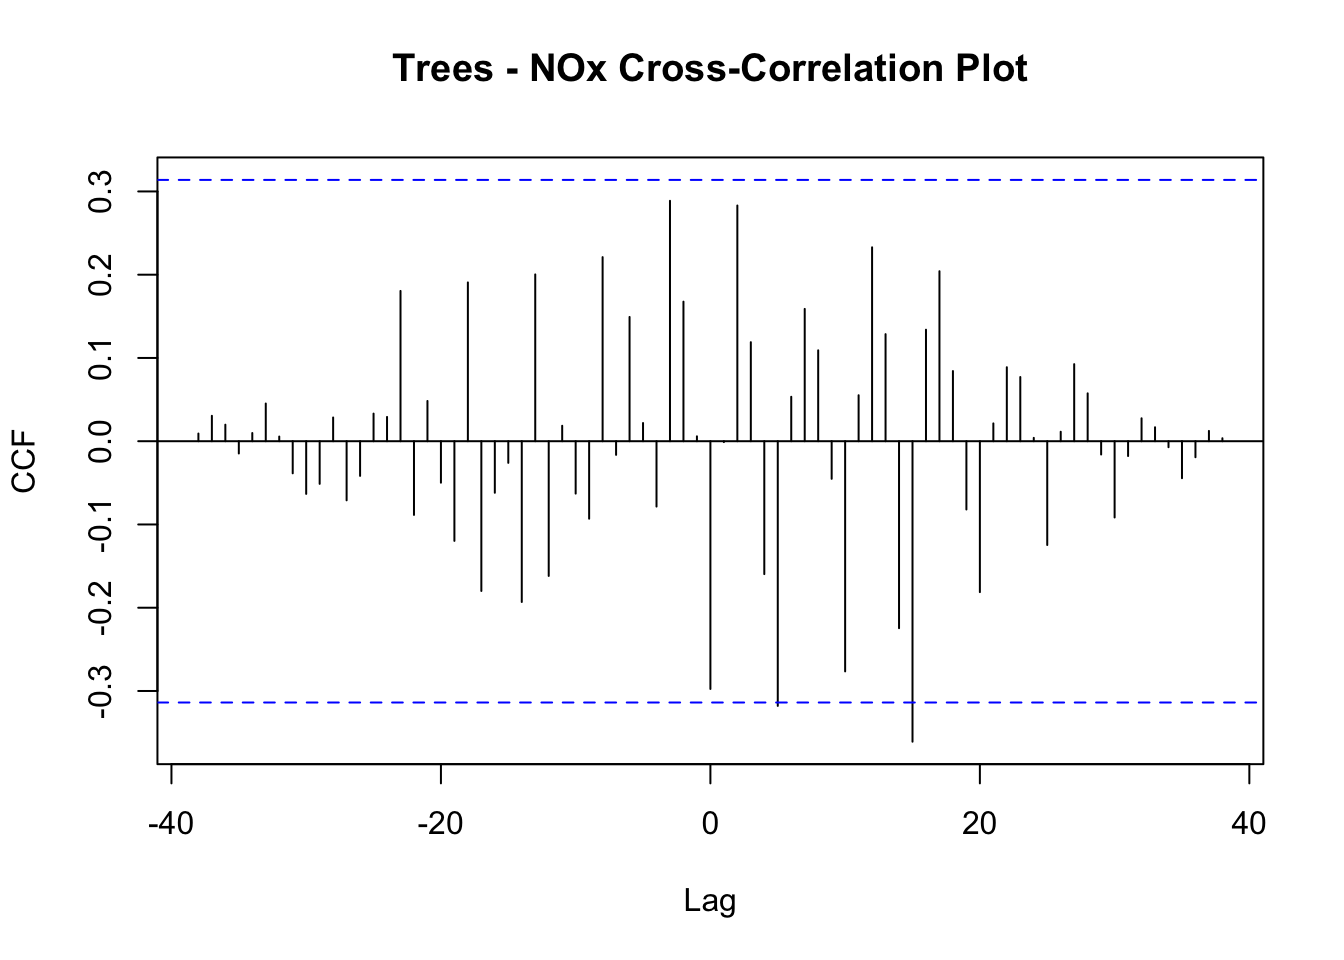
\includegraphics[width=0.33\linewidth]{sustainability_group_files/figure-latex/correlation-1} 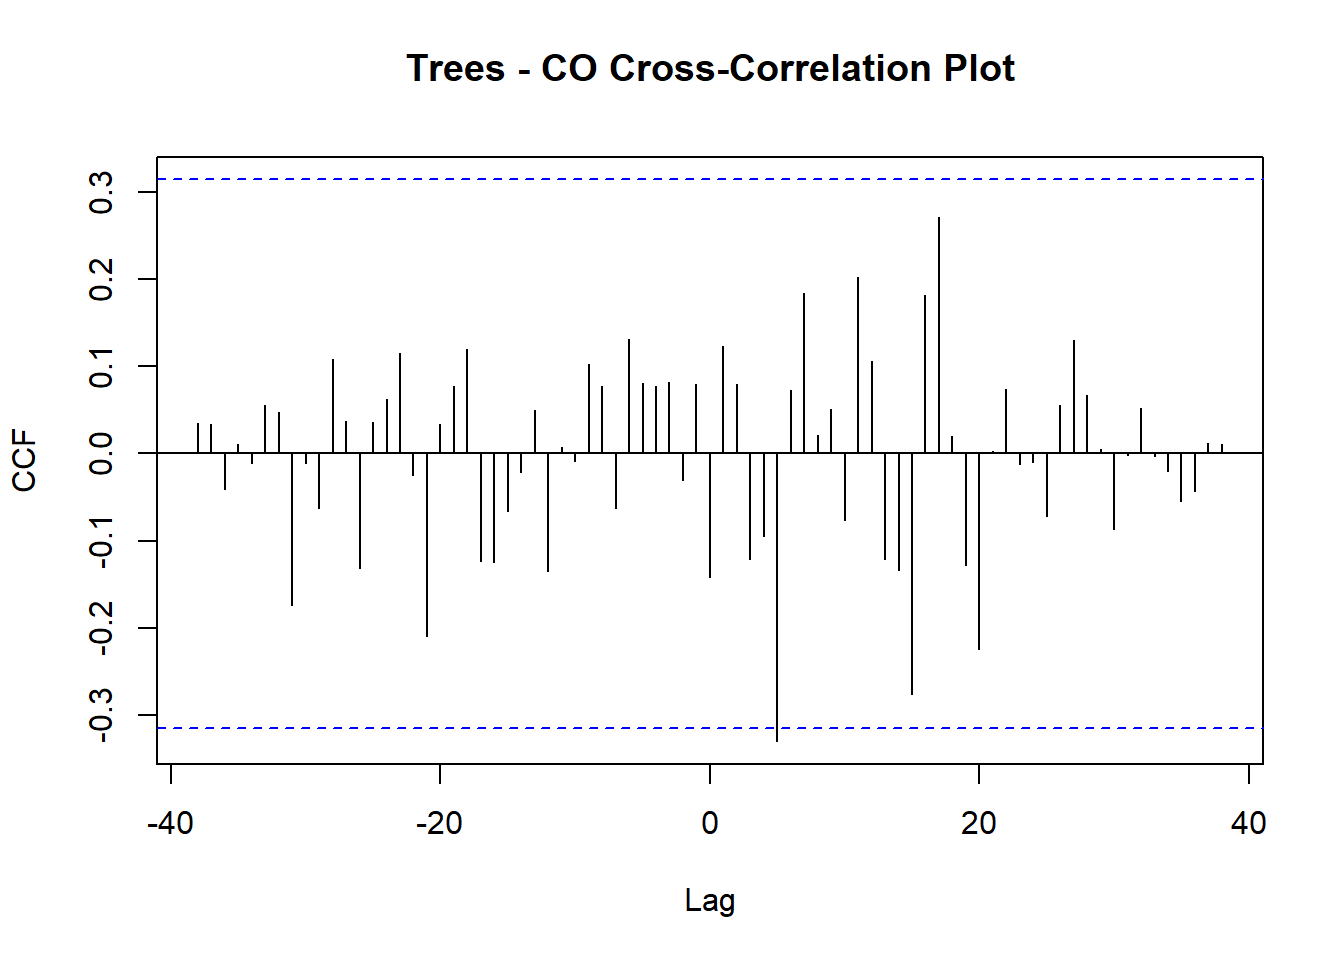
\includegraphics[width=0.33\linewidth]{sustainability_group_files/figure-latex/correlation-2} 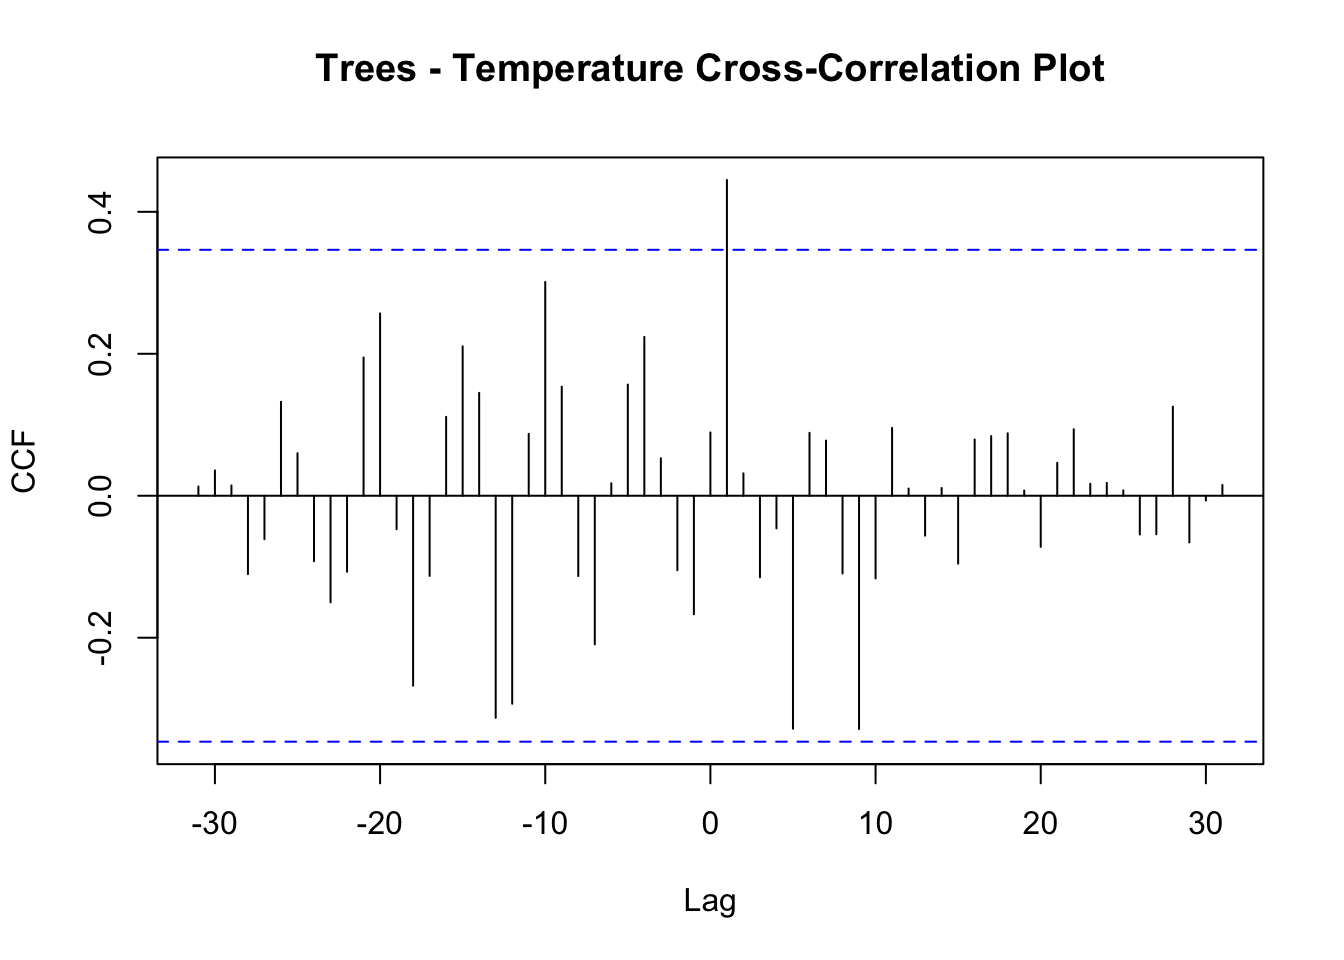
\includegraphics[width=0.33\linewidth]{sustainability_group_files/figure-latex/correlation-3} \caption{Fig. nnn: Correlation timeseries}\label{fig:correlation}
\end{figure}

Now one can see the correlations between the sum of trees and air
quality (CO and NOx) as well as the correlation between the sum of trees
and temperature. The graphs shows no strong correlations, although a
slightly significant correlation with a lag is visible for amount of
trees on air quality. Meaning that after a some time a larger amount of
trees could have an influence in reducing Carbon monoxide and Nitrogen
oxide in the air. To further analyse this more data from more measuring
station over a number of years would be necessary. The timeseries
analysis leads us to the conclusion that the impact of trees might be
very localized and shows that nearly no correlation between trees and
air quality or temperature is visible in the available data.

\hypertarget{tableau-dashboards}{%
\subsection{Tableau Dashboards}\label{tableau-dashboards}}

To aid us in our geospatial analysis and to potentially communicate some
of our findings to a broader public, we have created a Tableau
dashboard. The first visualization shows that

Below you can find a screenshot of one of the visualizations in our
dashboard. To explore the full interactive dashboard, please follow the
following link.

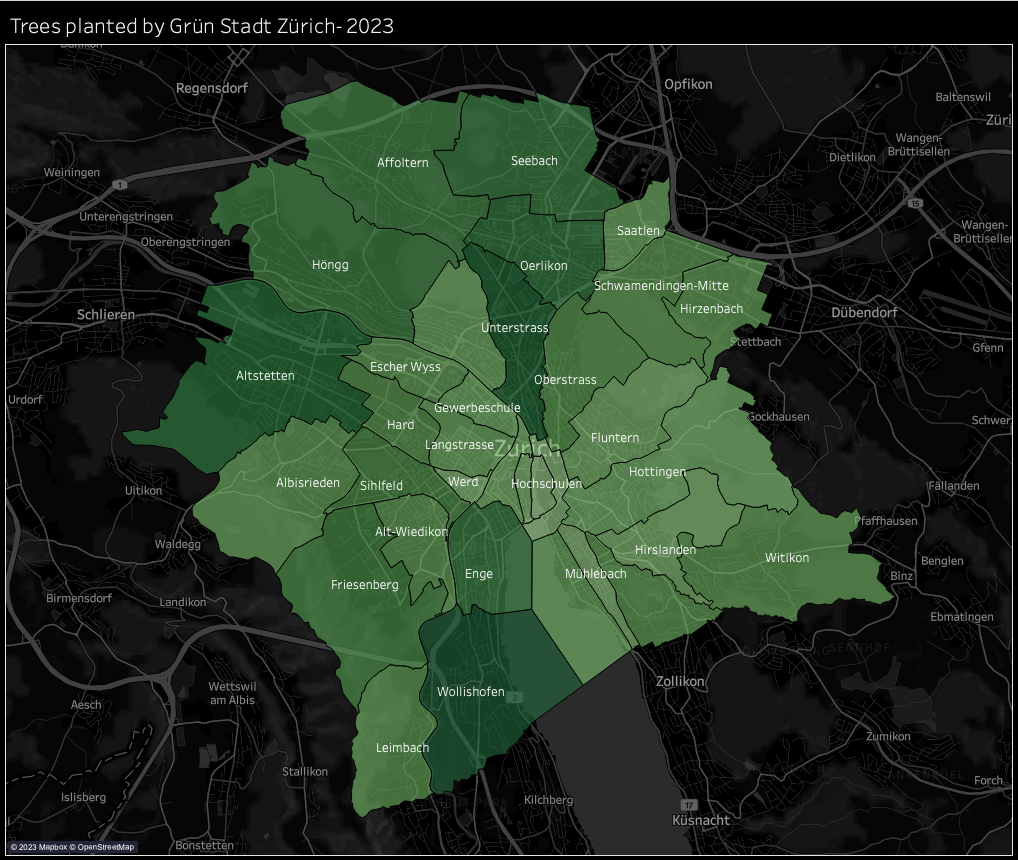
\includegraphics{../images/tableau_trees_total.png}\\
For the dashboard, some additional data wrangling was done. Furthermore
the dataset had to be expanded and missing values needed to be added to
create a smoother dashboard experience.

\begin{figure}
\centering
\includegraphics{sustainability_group_files/figure-latex/Tableau_data_wrangling-1.pdf}
\caption{Fig. 1: Text}
\end{figure}

\hypertarget{conclusions-and-findings}{%
\subsection{Conclusions and findings}\label{conclusions-and-findings}}

Based on our data, there is no correlation between the number of trees
planted in a given district in the city of Zurich and the temperature on
a macro scale. The same is true for the timeseries analysis between
number of trees and the air quality. It is likely that there are too
many additional factors outside of the data that influence it. The data
also shows that it is very probable that the effects of trees is very
localized and that the do not have an impact if they are too far away
from the measuring station. Thus we would recommend a very localized
experiment that removes as many outside factors as possible.

\hypertarget{outlook-and-next-steps}{%
\subsection{Outlook and next steps}\label{outlook-and-next-steps}}

While we did manage to get some very insightful and interesting results,
we did also come across some issues, mostly with the data availability
and quality. It would be useful to collect more data from across the
different districts in Zürich. It would also be helpful if that data
would be completely available across a time-frame of at least 20 years.
This would allow for creating a more complete picture and better
comparisons among districts. Another possibility would be take a closer
look at some of the outliers using Extreme Value Theory (EVT). A further
approach would be to create a simulation. While this would obviously
involve a lot more effort, it would allow to simulate potential
scenarios and could thus help city planners and politicians to make more
informed policy decisions.

Further research questions could evaluate the temperature on both a
micro and macro scale. Especially interesting would be an evaluation to
calculate or simulate the amount of vegetative cooling to reach a
critical mass that makes the efforts observable on a macro level. In our
opinion, it would be useful to not only include trees, as our research
did, but also plants on facades and rooftops. Furthermore, the study
should be controlled against the disappearance of undeveloped land in
favour of urban spread.

\end{document}
